\renewcommand{\thechapter}{\arabic{chapter}}
\setcounter{chapter}{4}

\chapter{Diagnostic de l'image}
\label{chap:chapter_5}
\chapterintro
Comme évoqué durant le préambule, cette partie s'impose comme une première étape au processus global de détection sur la modalité \gls{rcm}. En d'autres termes ce chapitre regroupe diverses méthodes relatives à la classification des images de cette modalité. Plus précisément, ces méthodes se consacrent à une séparation des images selon les annotations \textbf{saines}, \textbf{bénignes} ou \textbf{malignes} et répondent également à la détection d'images malignes.\par

Ainsi, ce chapitre propose une approche en plusieurs étapes. La première d'entre elles se destine à l'extraction de caractéristiques pertinentes par des méthodes manuelles mais également auto-déterminées à l'aide de réseaux profonds pré-entraînés, tandis que la seconde explore la mise en œuvre de méthodes de classification éprouvées. Afin de rendre plus riche cette partie et de compléter ses conclusions, la dernière étape aborde divers aspects tels que l'influence de paramètres liés à la normalisation des caractéristiques, la réduction de l'information dans le contexte de méthodes à fort nombre de dimensions ou encore l'influence des données sur les résultats de classification.\par	
\newpage

%%%%%%%%%%%%%%%%%%%%%%%%%%%%%%%%%% 
%%%%%%%%%%%%%%%%% METHODOLOGIE
\section{Méthodologie}
La classification de lésions de la peau, telles que le mélanome, par l'utilisation de méthodes d'apprentissage sont l'une des problématiques très largement développé de la littérature. Néanmoins, cette littérature se restreint à quelques articles de recherche~\cite{Halimi2017a, Halimi2017b, Wiltgen2008, Koller2011} lorsque que ce cadre se recentre en particulier sur la détection des pathologies de \gls{lm} et \gls{lmm} couplées à la modalité de \gls{rcm}. Pour cela, la détection de ces pathologies est réalisée à l'aide de la base d'images mise à disposition, essentiellement centrée autour de lésions malignes de \gls{lm} et \gls{lmm}. Divers angles d'approche sont ainsi menés, avec~: 
\begin{itemize}
    \item d'une part sous la forme d'une problématique à trois classes, la séparation des tissus \textbf{sains}, \textbf{bénins} et \textbf{malins},
    \item et d'autre part sous la forme d'une problématique binaire, la séparation entre les tissus \textbf{malins} et le \textbf{reste} des tissus.
\end{itemize}\par

Pour cela, ces deux situations sont abordées à l'aide de processus d'apprentissage supervisées dont les diverses étapes sont déroulées lors de ces prochains paragraphes. En effet, ces approches sont largement développées et démontrées fonctionnelles sur des thématiques variées du domaine de l'imagerie médicale et s'imposent pour la suite de ces travaux~\cite{Litjens2017,Pathan2018}. Ainsi, les étapes essentielles des processus de classification \textit{classiques} sont utilisées et adaptées à la problématique de ce manuscrit.\par

Le pré-traitement des images n'est pas considéré dans ce travail~: d'une part les images \gls{rcm} ne présentent que peu d'artefacts voire aberrations et d'autre part cet aspect est faiblement traité dans la littérature. De ce fait, le processus de classification se compose de trois étapes majeures~:
\begin{inlinerate}
    \item l'extraction de caractéristiques,
    \item le pré-traitement avant classification,
    \item et les méthodes de classification.
\end{inlinerate} La \Cref{fig:scheme_macro_image_classification} permet une vision globale de ce processus de classification. Ainsi, une section est respectivement dédiée à chacune de ces trois étapes, puis à l'aide de deux sections distinctes sont présentés les résultats de ces expérimentations et leur analyse.\par

\begin{figure}[H]
\centering
    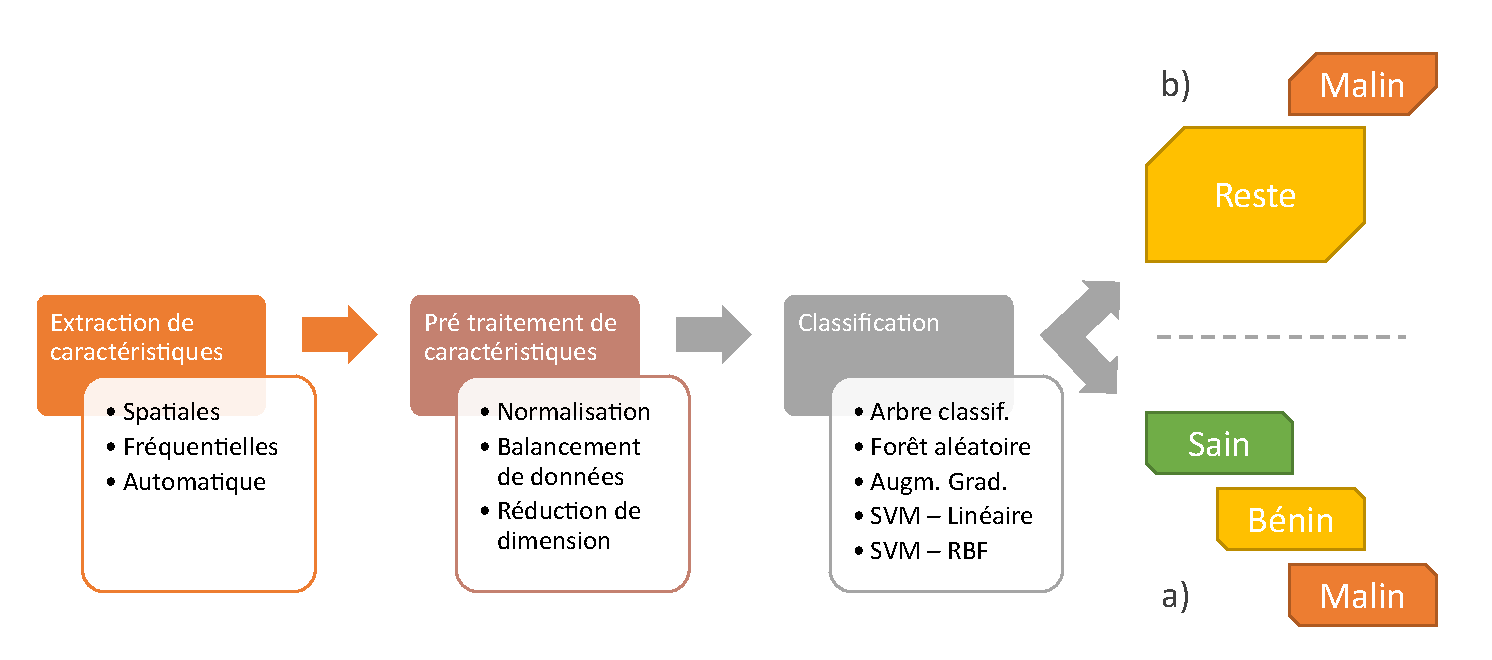
\includegraphics[width=\linewidth]{contents/chapter_5/resources/scheme_macro_image_classification.pdf}
    \caption{Représentation du processus de diagnostic suivi dans le cadre de l'apprentissage automatique pour les images \gls{rcm}. Ce processus permet une prédiction à trois classes - a), mais également binaire en se focalisant sur la détection de la classe maligne - b).}
    \label{fig:scheme_macro_image_classification}
\end{figure}\par

\newpage

%%%%%%%%%%%%%%%%%%%%%%%%%%%%%%%%%% 
%%%%%%%%%%%%%%%%% FEATURES
\section{Méthodes d'extraction de caractéristiques}
\label{chap:feature_extraction}
L'étape d'extraction de caractéristiques consiste en l'obtention de valeurs dérivées à partir des données brutes dans le but de quantifier un phénomène. Ces valeurs jugées pertinentes sont ensuite utilisée pour la suite du traitement, généralement de la classification. Les éléments présentés en préambule visent à montrer l'importance des motifs de tissus, dont l'apparence varie selon~:
\begin{itemize}
    \item \textbf{la profondeur de l'acquisition} du tissus considéré, ainsi l'épiderme, \gls{dej} et le derme sont très différents du point de vue des tissus qui les constituent,
    \item \textbf{la pathologie à identifier}, les différentes lésions en notre possession sont assez différentes selon leur état bénin ou malin.
\end{itemize}
Les nombreux échanges, menés auprès de dermatologues visant à l'introspection de leur propre processus cognitif lors de la décision, aboutissent à une forte présomption de l'importance de \textbf{la texture} des tissus présents dans ces images.\par

Les méthodes d'extraction de caractéristiques sont abordées selon deux axes~:
\begin{inlinerate}
    \item d'une part, les \textbf{méthodes \textit{manuelles} d'extraction de caractéristiques} ou déterminées par un humain respectivement séparées en caractéristiques \textit{spatiales} et \textit{fréquentielles},
    \item d'autre part, les \textbf{méthodes \textit{non manuelles} d'extraction de caractéristiques}.
\end{inlinerate} 
L'appellation \textit{manuelle} s'est ainsi imposée suite à l'apparition de réseaux de convolution profonds, afin de distinguer ces deux types d'approches~\cite{Nanni2017}.\par

\subsection{Méthodes manuelles d'extraction de caractéristiques spatiales}
L'extraction sur base d'information du domaine spatial est un champ de travail assez développé présentant comme avantage d'être intuitif mais pouvant être affecté par le bruit et autres phénomènes de dégradation de l'information. Ces opérations spatiales peuvent être décrites à deux niveaux d'interprétation, d'une part celui des valeurs brutes dont les descripteurs de premier ordre font partie mais ne fournissent aucune valeur de cohérence spatiale et, d'autre part celui par transformation de l'information initiale dont les descripteurs de second ordre ou plus font partie. Ces dernières méthodes prennent en compte la relation d'une valeur locale à celle de son voisinage~\cite{Kamila2015}.\par

Les descripteurs de premier ordre s'appliquent ainsi aux valeurs d'intensité ou à la distribution de celles-ci, sans traitement préalable. La \Cref{tab:first_order_descriptors} recense la plupart de ces caractéristiques issues de la distribution des valeurs brutes. Néanmoins, ces mesures tendent à ressortir des phénomènes globaux de l'image, mais ne suffisent pas à elles seules à analyser des motifs présents~\cite{Tomita1990, Srinivasan2008, Uyun2013, NyeinNyeinHlaing2015}. Ces mesures ont notamment été utilisées comme un complément de classification~\cite{Wiltgen2008}.\par

\begin{table}[H]
    \centering
    \begin{tabular}{ll}
        \toprule
        \textbf{Mesure}             & \textbf{Expression mathématique}                                                  \\ \hline
        Moyenne                     & $\overline{x} = \frac{1}{n}\sum_{i=1}^n x_i$                                      \\   
        Variance                    & $v = \frac{1}{n}\sum_{i=1}^n \left(x_i - \overline{x}\right)^2$                   \\ 
        Entropie                    & $e = -\sum_{i=1}^n {\mathrm{P}(x_i) \log_b \mathrm{P}(x_i)}$                      \\
        Kurtosis                    & $k=\frac{r \sum_{i=1}^{n}\left(x_{i}-\bar{x}\right)^{4}}{\left(\sum_{i=1}^{n}\left(x_{i}-\bar{x}\right)^{2}\right)^{2}}-3$\\
        Asymétrie                   & $a = \mathbb{E} \left[ \left( \frac{X - \mu}{\sigma} \right)^3 \right]$           \\  
        \bottomrule
    \end{tabular}
    \caption{Liste de différentes mesures obtenues à partir du premier ordre.}
    \label{tab:first_order_descriptors}
\end{table}\par

Les descripteurs de second ordre, ou plus, utilisent l'information locale et en déduisent une relation à leur voisinage par l'utilisation d'une transformation intermédiaire. Parmi ces transformations, les plus courantes d'entre elles sont~: 
\begin{inlinerate}
    \item la \gls{glcm},
    \item la \gls{glrlm},
    \item et la \gls{glszm}.
\end{inlinerate} 
L'extraction sur la base d'information du second ordre a notamment été traitée en 1973 pour de la reconnaissance sur des images aériennes et satellites, par Haralick et al.~\cite{Haralick1973}. Ce travail est une extension des \gls{glcm}, dont le principe consiste en un recensement des combinaisons d'intensité présentes dans une image. Cette extraction nécessite une direction dans laquelle les combinaisons sont recherchées, en 2D ces directions sont aux nombres de quatre~:
\begin{inlinerate}
    \item horizontale,
    \item verticale,
    \item et les deux diagonales opposées.
\end{inlinerate}
Le principe de fonctionnement des \gls{glcm} est schématisé en \Cref{fig:scheme_principle_GLCM} pour une extraction selon la direction horizontale. Le travail~\cite{Haralick1973} a ainsi démontré la pertinence des \gls{glcm} dans la différenciation d'images texturées, en calculant selon les quatre directions évoquées précédemment, quatorze critères statistiques. Ces divers critères statistiques sont recensés sur la \Cref{tab:haralick_descriptors}, ainsi que leurs formules associées. La bibliothèque logicielle \textit{Mahotas}~\cite{coelho2012} est utilisée afin de réaliser ces diverses extractions de manière optimale et dans un temps raisonnable.\par
 
\begin{figure}[H]
    \centering
    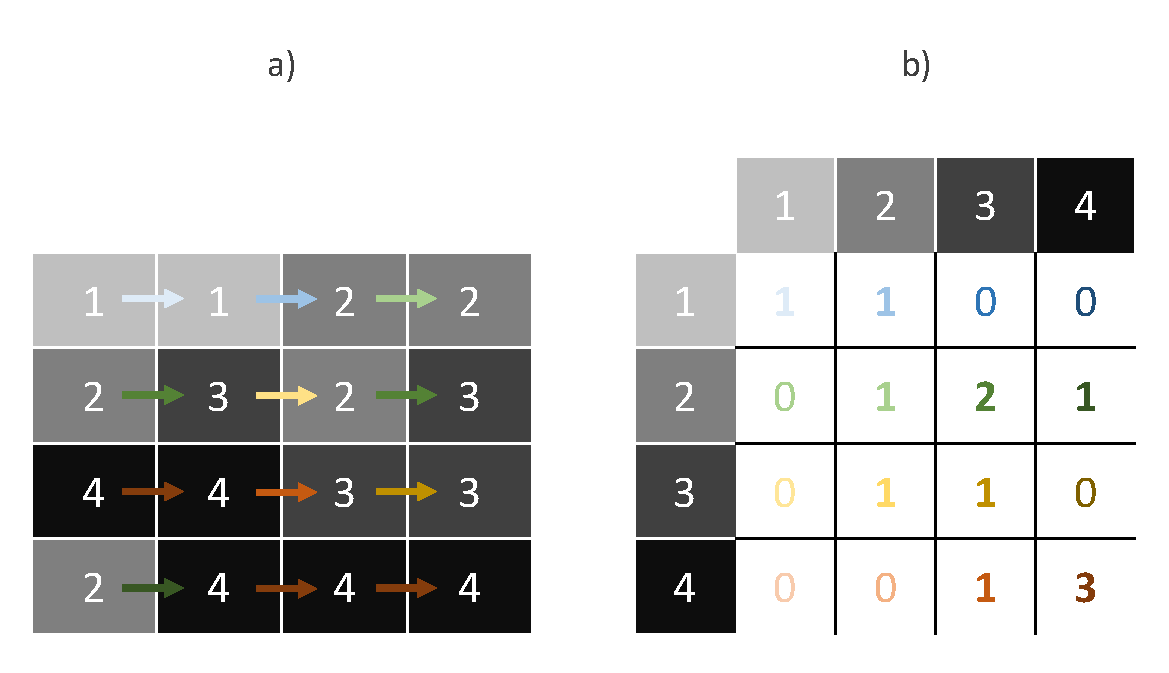
\includegraphics[width=\linewidth]{contents/chapter_5/resources/scheme_principle_GLCM.pdf}
    \caption{Représentation de la création d'une matrice sur base de \gls{glcm} selon la direction horizontale et dont la valeur de distance de voisinage est de 1. En a), les flèches représentent les diverses relations de voisinage horizontal caractérisés par une couleur ; En b), ces diverses relations sont recencés dans la matrice de \gls{glcm} en employant les même codes de couleurs.}
    \label{fig:scheme_principle_GLCM}
\end{figure}\par

Les travaux menés par l'une des études sur les lésions mélanocytaire en \gls{rcm}~\cite{Wiltgen2008}, complètent ces deux catégories de mesures spatiales par de l'information de texture. En effet, l'étude met en avant l'importance des douze premières caractéristiques formulées par Haralick~\cite{Haralick1973} et adjoint cinq mesures de premier ordre comme complément d'information dont~:
\begin{inlinerate}
    \item la moyenne,
    \item l'erreur quadratique moyenne,
    \item l'asymétrie de la répartition de l'histogramme,
    \item le kurtosis (mesure d'aplatissement de la distribution),
    \item et l'entropie.
\end{inlinerate}
Ce même travail met en avant que la texture des lésions de la peau ne possède pas d'orientation particulière. Afin de rendre ces caractéristiques plus robustes aux rotations et, de réduire la quantité d'informations extraite, ses auteurs préconisent l'utilisation d'une moyenne sur les quatre directions. Ainsi, cette manipulation permet de réduire l'information à un unique vecteur de taille 1$\times$12 pour ces caractéristiques d'Haralick~\cite{Wiltgen2008}.\par

\begin{table}[H]
    \centering
    \begin{tabular}{ll}
        \toprule
        \textbf{Mesure}                     & \textbf{Expression mathématique}                                                              \\ \hline
        Moment Angulaire                    & $ \sum_i\sum_jp(i,j)^2$                                                                       \\
        Contraste                           & $\sum_{k=0}^{N_g-1} k^2 p_{x-y}(k)$                                                           \\
        Corrélation                         & $\frac{\Large{\sum_{i=1}^{N_g}\sum_{j=1}^{N_g}} (ij)p(i,j) - \mu_x\mu_y}{\sigma_x\sigma_y}$   \\
        Différence des Moments Inverse      & $\sum_{i=1}^{N_g}\sum_{j=1}^{N_g} \frac{1}{1 + (i - j)^2} p(i,j)$                             \\   
        Entropie                            & $-\sum_{i=1}^{N_g}\sum_{j=1}^{N_g} p(i,j) \log(p(i,j))$                                       \\   
        Somme - Moyenne                     & $\sum_{i=2}^{2N_g} i p_{x+y}(i)$                                                              \\    
        Somme - Variance                    & $\sum_{i=2}^{2N_g} (i - f_8)^2 p_{x+y}(i)$                                                    \\    
        Somme - Entropie                    & $\sum_{i=2}^{2N_g} (i - f_8)^2 p_{x+y}(i)$                                                    \\    
        Somme des carrés - Variance         & $\sum_{i=1}^{N_g}\sum_{j=1}^{N_g} (i - \mu)^2 p(i,j)$                                         \\   
        Différence - Variance               & ${\rm variance \ of ~} p_{x-y}$                                                               \\    
        Différence - Entropie               & $-\sum_{i=0}^{N_g-1} p_{x-y}(i) \log(p_{x-y}(i))$                                             \\
        Mesure de Corrélation 1             & $\frac{f_9 - HXY1}{\max(HX,HY)}$                                                              \\  
        Mesure de Corrélation 2             & $[1 - \exp(-2(HXY2 - f_9))]^{1/2}$                                                            \\ 
        Coefficient de Corrélation Maximal  & $(max(\sum_k \frac{p(i,k)p(j,k)}{p_x(i)p_y(k)}))^{1/2}$                                       \\ 
        \bottomrule
    \end{tabular}
    \caption{Liste des différentes mesures proposée par Haralick et al.~\cite{Haralick1973} applicables aux \gls{glcm} pour caractériser des images texturées.}
    \label{tab:haralick_descriptors}
\end{table}\par
 
Les expériences menées sur base de descripteurs manuels spatiaux se décomposent en plusieurs temps. Tout d'abord, l'importance de l'information de \textbf{premier ordre} et de second ordre proposée par \textbf{Haralick} selon les \textit{quatre directions} mais aussi la \textit{moyenne} sont évaluées sur leur aptitude à séparer les divers groupes de données. Enfin, la méthode de \textbf{Wiltgen} et al. qui propose la combinaison de ces deux précédentes technique est évaluées en ces même termes~\cite{Wiltgen2008}. Par ailleurs, la \Cref{tab:number_features_spatial} synthétise l'ensemble des méthodes d'extraction ainsi que le nombre associé de caractéristiques extraites.\par
\begin{table}[h]
    \centering
    \begin{tabular}{ll}
        \toprule
        \textbf{Méthode}                            & \textbf{Nombre de caractéristiques}   \\ \hline
        Mesures premier ordre                       & 14                                    \\ \hline
        Haralick~\cite{Haralick1973} - 4 directions & 56                                    \\ \hline
        Haralick~\cite{Haralick1973} - Moyenne      & 14                                    \\ \hline
        Wiltgen~\cite{Wiltgen2008} - Spatial        & 17 (12+5)                             \\
        \bottomrule                 
    \end{tabular}
    \caption{Liste des méthodes spatiales évaluées dans ce chapitre et leur nombre de caractéristiques extraites associées.}
    \label{tab:number_features_spatial}
\end{table}
\clearpage

\subsection{Méthodes manuelles d'extraction de caractéristiques fréquentielles}
L'extraction sur base d'information du domaine fréquentiel est également un champ de travail assez développé, notamment pour sa robustesse face aux perturbations telles que le bruit, ainsi que la vitesse d'exécution de certaines opérations telles que le filtrage. En revanche, l'information extraite est plus difficile d'interprétation et, nécessite une information spatiale suffisamment conséquente pour être juste~\cite{Kamila2015}. Ce dernier point est négligeable dans ce travail, les données de \gls{rcm} exploitées dans le cadre de ces travaux étant dotées d'une résolution spatiale suffisante de \SI{1000}{\px} $\times$ \SI{1000}{\px}.\par

Plusieurs courants majeurs de représentation fréquentielle sont utilisés, dont~: 
\begin{itemize}
    \item la Transformée de Fourier~\cite{Ursani2007, Smach2008a},
    \item la Transformée en cosinus discrète~\cite{Sorwar2001},
    \item la Transformée en ondelettes~\cite{Arivazhagan2003,Hong2010},
    \item et la Transformée de Gabor~\cite{Ursani2007}.
\end{itemize}
Ce travail se consacre à deux de ces approches, d'une part à la transformée de Fourier et d'autre part à la transformée en ondelettes, toutes deux traitées sur des problématiques de classification similaires~\cite{Wiltgen2008,Halimi2017a,Halimi2017b}. Également, ces deux méthodes sont deux représentants majeurs des deux grandes familles de représentation en fréquences.\par

\begin{figure}[h]
    \begin{center}
        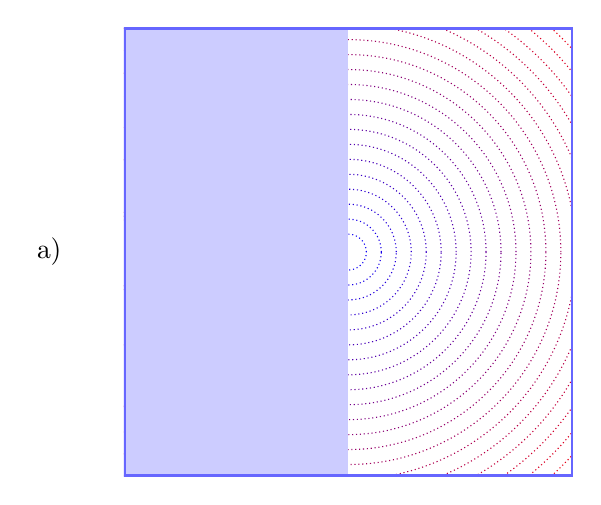
\begin{tikzpicture}[scale=1.9]
            \node[] at (-2, 0) {a)};
            \begin{scope}
                \clip (-1.5, -1.5) rectangle (1.5, 1.5);
                \foreach \cRadius in {1, ..., 22}
                    \pgfmathsetmacro\cColor{\cRadius/22*100}
                    \draw[red!\cColor!blue, densely dotted] (0, 0) circle (0.02+\cRadius*0.1); 
                    
                \fill[blue!20] (-1.5, -1.5) rectangle (0, 1.5);
                \draw[blue!60, ultra thick] (-1.5, -1.5) rectangle (1.5, 1.5);
            \end{scope}
        \end{tikzpicture}
        \qquad
        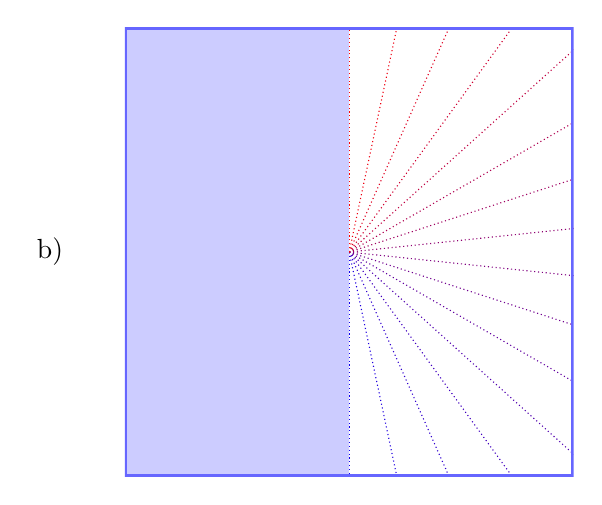
\begin{tikzpicture}[scale=1.9]
            \node[] at (-2, 0) {b)};
            \begin{scope}
                \clip (-1.5, -1.5) rectangle (1.5, 1.5);
                \foreach \cAngle in {1, ..., 16}
                    \pgfmathsetmacro\cColor{\cAngle/16*100}
                    \draw[red!\cColor!blue, densely dotted] (0, 0) -- (\cAngle* 180 / 15 -102:3); 
                \fill[blue!20] (-1.5, -1.5) rectangle (0, 1.5);
                \draw[blue!60, ultra thick] (-1.5, -1.5) rectangle (1.5, 1.5);
            \end{scope}
        \end{tikzpicture}
    \end{center}
    \caption{Schéma représentant l'extraction de caractéristiques à partir de l'espace de Fourier. En a), l'utilisation de cercles concentriques depuis l'origine, schématisé en pointillés ; En b), l'extraction selon une direction.}
    \label{fig:scheme_fourier_features}
\end{figure}\par

La transformée de Fourier se résume à la décomposition d'une donnée en une somme de fréquences. Dans le cas d'une image, cette transformation donne lieu à une représentation, dans laquelle les basses fréquences, au centre, représentent une forme d'homogénéité au sein d'une image tandis que les hautes fréquences, en extérieur, sont associées à de fortes zones de transitions. Cette transformation conserve également l'orientation des fréquences, représentée à l'aide d'un angle formé à partir de l'origine. En revanche, bien que la transformée de Fourier permette de décrire parfaitement la composition fréquentielle de l'image, elle ne peut en localiser la provenance des fréquences~\cite{Wiltgen2008}. Cet espace reste néanmoins approprié à la caractérisation d'images texturées, et a suscité un grand intérêt au milieu des années 1980~\cite{Persoon1986}. Différentes mesures ont été proposées dans cet espace afin de caractériser des textures~:
\begin{itemize}
    \item l'extraction d'information à partir \textbf{de cercles concentriques} réguliers~\cite{Smach2008a, Wiltgen2008} afin d'isoler l'information propre à chaque intervalle de fréquences (\Cref{fig:scheme_fourier_features} - a),
    \item l'extraction d'information à partir \textbf{de directions} en partance du centre vers l'extérieur de la transformée à angles constants~\cite{Wiltgen2008} (\Cref{fig:scheme_fourier_features} - b).
\end{itemize}
Ces deux travaux préconisent l'extraction d'une valeur de moyenne et d'un écart-type sur différentes régions de l'espace fréquentiel afin de qualifier les phénomènes précédemment présentés~\cite{Smach2008a, Wiltgen2008}. 

L'une des expériences menée par Wiltgen et al.~\cite{Wiltgen2008} se base sur la transformée de Fourier, et extrait \textbf{38 descripteurs} du spectre de magnitude~:
\begin{itemize}
    \item \textbf{22 descripteurs} correspondent à la moyenne calculée sur des rayons répartis de manière équidistante du centre du spectre (\Cref{fig:scheme_fourier_features} - a),
    \item \textbf{16 descripteurs} correspondent à la moyenne calculée sur des directions à intervalles constants (\Cref{fig:scheme_fourier_features} - b).
\end{itemize}
La transformée de Fourier est effectuée dans le reste de ce travail par la bibliothèque logicielle \textit{SciPy} \cite{Virtanen2020}.\par

\begin{figure}[H]
    \centering
    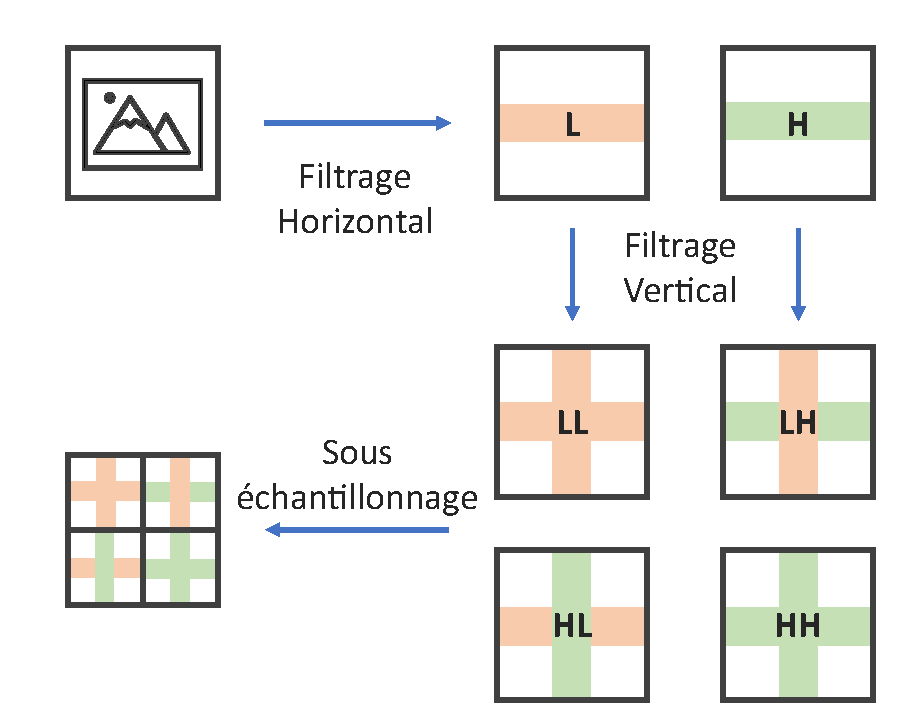
\includegraphics[width=0.75\textwidth]{contents/chapter_5/resources/scheme_dwt.pdf}
    \caption{Principe de la décomposition en ondelettes appliquée aux images~\cite{Livens1997}. La décomposition est réalisée en trois temps. Un filtrage passe bas (L) et passe haut (H) sont réalisés selon la direction horizontale, puis selon la direction verticale. Enfin, un sous échantillonnage de coefficient 2 est appliqué afin d'obtenir une matrice de même taille que l'image d'origine.}
    \label{fig:scheme_dwt}
\end{figure}\par 

La transformée en ondelettes possède divers avantages dont une bonne capacité de localisation, par translation de l'ondelette mère, et la possibilité de prendre en considération plusieurs échelles d'analyse, par homothétie~\cite{Livens1997,Wiltgen2008}. Concernant le choix de l'ondelette mère, celui-ci ne semble pas affecter la qualité des caractéristiques extraites~\cite{Fatemi1996, Livens1997} bien que, l'un des auteurs préconise le choix d'ondelettes symétriques ou anti-symétriques~\cite{Livens1997}. Néanmoins, les ondelettes de Daubechies et de Haar sont privilégiées lors de ces diverses expérimentations fréquentielles, les diverses références littéraires s'orientant vers  celles-ci~\cite{Wiltgen2008,Halimi2017a}. La décomposition en ondelettes sur images se réalise en trois étapes successives~: 
\begin{inlinerate}
    \item de filtrage passe-bas et passe-haut horizontal,
    \item de filtrage passe-bas et passe-haut vertical,
    \item puis une étape de sous-échantillonnage afin de réduire la quantité d'informations généré après ces deux précédentes étapes.
\end{inlinerate} Ce processus en trois temps est schématisé sur la \Cref{fig:scheme_dwt} et les opérations de transformée en ondelettes sont effectuées à l'aide de la bibliothèque logicielle \textit{PyWavelets}~\cite{lee2006}.\par

Ainsi, les expériences sur la base de descripteurs en fréquences sont réalisées en plusieurs temps. Dans un premier temps, la performance de la transformation de \textbf{Fourier} et de la transformation en ondelettes de \textbf{Daubechies} mais également de \textbf{Haar} est mesurée sur la séparation des divers groupes d'images. Dans un second temps, la méthode de \textbf{Wiltgen} et al. employant une combinaison de descripteurs de l'espace de Fourier est évaluée dans ces même conditions~\cite{Wiltgen2008}. La \Cref{tab:number_features_frequency} synthétise le nombre associé de caractéristiques extraites par ces diverses méthodes d'extraction fréquentielles.\par

\begin{table}[H]
    \centering
    \begin{tabular}{ll}
        \toprule
        \textbf{Méthode}                        & \textbf{Nombre de caractéristiques}   \\ \hline
        Fourier                                 & 10 / 20 / 30                          \\ \hline
        Ondelettes de Daubechies                & 12                                    \\ \hline
        Ondelettes de Haar                      & 12                                    \\ \hline
        Wiltgen~\cite{Wiltgen2008} - Fourier    & 38 (22+16)                             \\
        \bottomrule
    \end{tabular}
    \caption{Liste des méthodes fréquentielles évaluées dans ce chapitre et leur nombre de caractéristiques extraites associées.}
    \label{tab:number_features_frequency}
\end{table}\par
\clearpage

\subsection{Méthode d'apprentissage par transfert de connaissances}
Les méthodes d'apprentissage par transfert de connaissances sont un champ d'application relativement récent de l'apprentissage automatique. Le principe est de réutiliser des connaissances précédemment acquises, dans le but de résoudre de nouveaux problèmes plus rapidement, voire plus efficacement. Pour cela, ce champs vise à proposer des techniques permettant la transposition de connaissances d'une ou plusieurs tâches sources à une tâche cible~\cite{QiangYang2010}.\par

Le phénomène conjoint d'engouement pour les \gls{cnn} et la complexité des architectures récentes pour le traitement des images a accentué les recherches en ce sens. En effet, les techniques d'apprentissage par transfert de connaissances sont une réponse efficace à de nombreuses problématiques autour de l'entraînement des \gls{cnn}, comme~: 
\begin{itemize}
    \item les \textbf{contraintes de suffisance de données}, notamment de données convenablement structurées et annotées disponibles publiquement,
    \item le \textbf{complexité de l'entraînement}, comprenant le réglage des divers paramètres de ces réseaux (augmentations des données, fonction d'optimisation, \ldots),
    \item et les \textbf{contraintes matérielles nécessaires}, regroupant les aspects matériels dédiés au support de l'entraînement de ces architectures.
\end{itemize}\par

Certains domaines d'application ont vu apparaître de nombreuses bases de données publiques, contribuant à résoudre partiellement la contrainte liée aux données et permettant la mesure des performances de système de traitement de l'image. Parmi celles-ci, peuvent être citées~: 
\begin{inlinerate}
    \item la \textbf{base MNIST}, pour mesurer l'aptitude de systèmes dédiés à la reconnaissance de chiffres écrits à la main~\cite{lecun2010},
    \item les \textbf{bases CIFAR10 et CIFAR100}, permettant l'évaluation de systèmes de reconnaissance d'objets sur des image miniatures~\cite{Krizhevsky}, 
    \item et plus récemment, la \textbf{base ImageNet} pour la reconnaissance d'objets sur des images de taille commune~\cite{Deng2008}. 
\end{inlinerate}\par

Actuellement, la base ImageNet est l'une des plus sollicitées pour entraîner et évaluer les architectures de \gls{cnn} actuelles. Outre sa taille, cette base propose des niveaux d'annotations variées, dont 1000 classes sont proposées. De plus, une très grande diversité d'échantillons est mise à disposition pour chaque classe pour un total de plus de 14 millions d'images. Selon certaines études, ce nombre d'images reste néanmoins sur-dimensionné vis-à-vis du nombre d'éléments nécessaires à l'entraînement de ces réseaux~\cite{Huh2016}.\par

Parallèlement à ce phénomène de mise à disposition de bases de données, sont ouverts publiquement des défis visant à démontrer l'efficacité de chaînes de traitement pour gérer ces données. De nombreuses avancées ont été réalisées sur la base ImageNet, à l'aide d'architectures de \gls{cnn} régulièrement mises à disposition de la communauté. Parmi ces réseaux peuvent être cités les réseaux AlexNet~\cite{Krizhevsky2012}, GoogLeNet~\cite{Szegedy2015}, VGG~\cite{Simonyan2014}, Inception-V3~\cite{Szegedy2016}, ResNet~\cite{He2016} et Inception-ResNet~\cite{Szegedy2017}, avec respectivement comme précisions 0,54, 0,68, 0,71, 0,76, 0,78, and 0,80 sur la base ImageNet~\cite{Canziani2016}.\par

Néanmoins, la mise à disposition de la communauté de ces bases de données massives et de ces architectures ne permet pas de lever les deux verrous liés au contraintes d'entraînement et matérielles de ces réseaux. C'est donc particulièrement le partage de modèles de \gls{cnn} pré-entraînés, couplé aux principes d'apprentissage par transfert de connaissances, qui a suscité l'intérêt de nombreux travaux dont certains appliqués à l'imagerie médicale~\cite{Litjens2017}. Ainsi, la majeure partie de ces réseaux pré-entraînés est obtenu à l'aide de la base ImageNet, bien qu'aucune justification formelle n'ait été fournie à ce propos~\cite{Huh2016}.\par
 
\begin{figure}[H]
    \centering
    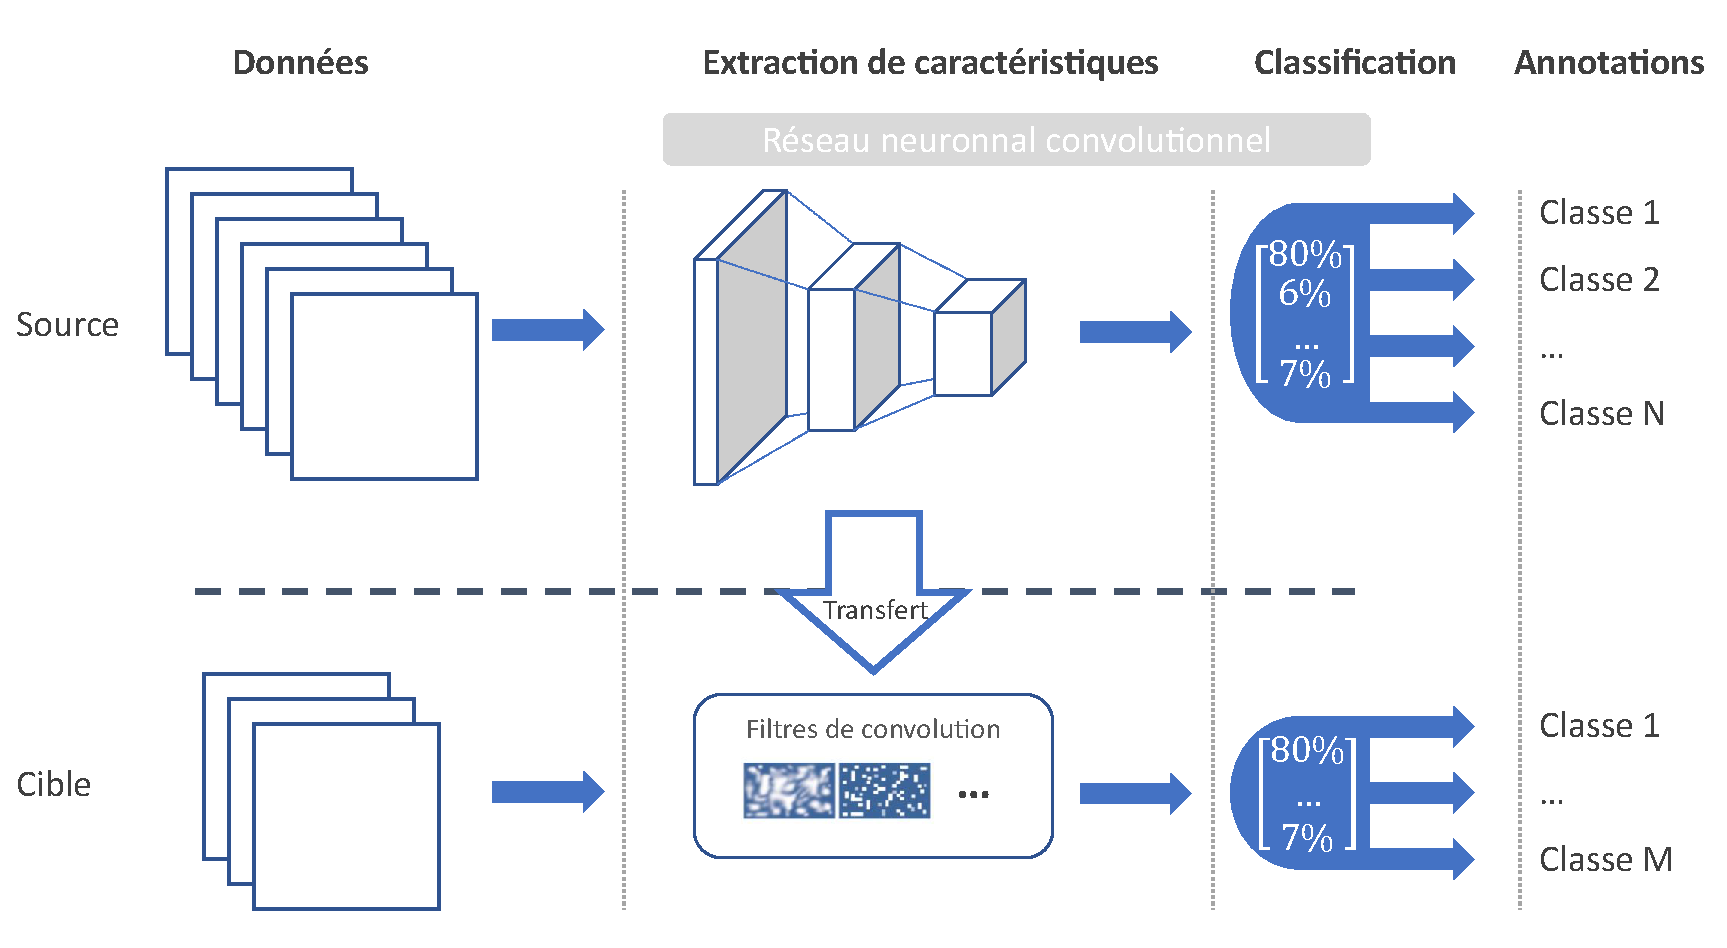
\includegraphics[width=\linewidth]{contents/chapter_5/resources/scheme_transfer_learning.pdf}
    \caption{Schéma représentant l'apprentissage par transfert par \gls{cnn}. Le réseau est entraîné sur des données et annotations d'une problématique \textit{source}. Puis, les paramètres de la partie liée à l'extraction de caractéristiques sont réemployés au sein d'une nouvelle problématique \textit{cible}.}
    \label{fig:scheme_transfer_learning}
\end{figure}\par

L'apprentissage par transfert sur \gls{cnn} se décompose en deux procédés majeurs~: 
\begin{inlinerate}
    \item d'une part, \textbf{l'extraction de caractéristiques} moins coûteuse en ressources matérielles et temps,
    \item et d'autre part, \textbf{le réglage fin} qui nécessite à l'inverse plus de temps et de ressources matérielles. 
\end{inlinerate}
Au sein de cette partie, le principe d'extraction de caractéristiques est développé afin de limiter les contraintes d'apprentissage, schématisée sur la \Cref{fig:scheme_transfer_learning}. Le principe consiste dans un premier temps à retirer les couches responsables de la classification du problème cible, puisque spécifiques au problème initial. Ces couches sont généralement des couches dites totalement connectées, qui vont pondérer l'importance des zones d'activation jusqu'aux classes respectives. Dans un second temps, les couches responsables de l'extraction de caractéristiques sont conservées puis figées, en partant du postulat que ces caractéristiques sont suffisamment variées et adaptées à d'autres problématiques du traitement d'image. Enfin, ces couches sont combinées à de nouvelles couches totalement connectées ou à des modèles de classification~\cite{Litjens2017}.\par 

A cette fin, une première stratégie consiste à aplatir l'information des couches d'extraction par une étape de \textit{Flatten} (littéralement \textit{Applatissement}), transformant celle-ci d'un format de matrice 3D à un vecteur 1D (voir \Cref{fig:scheme_global_pooling} - Gauche). Néanmoins, l'une des problématiques résultantes concerne la dimension spatiale souvent importante de ces caractéristiques extraites. En effet, la dimension spatiale de ces données sera réduite par les couches convolutionelles selon leurs paramètres dépendants de l'architecture choisie. Ainsi, les paramètres de décalage, de pas ou encore de taille du noyau de convolution sont autant de paramètres qui affectent la dimension spatiale de sortie. Pour pallier cette information conséquente, des couches dites de \textit{Global Pooling} ont été introduites dans la littérature, et consistent à réduire l'information spatiale d'une carte d'activation à une unique valeur dont le principe est schématisé sur la \Cref{fig:scheme_global_pooling} - Droite. Les principales fonctions mises à disposition sont la fonction maximum et moyenne, donnant respectivement lieu à des couches de \textit{Global Maximum Pooling} (ou \textit{Global Pooling - Maximum}) et de \textit{Global Average Pooling} (ou \textit{Global Pooling - Moyen}). D'autres fonctions sont également développées, mais la littérature s'accorde à préférer l'utilisation des couches de \textit{Global Pooling - Maximum}~\cite{christlein2019}.\par

\begin{figure}[H]
    \centering
    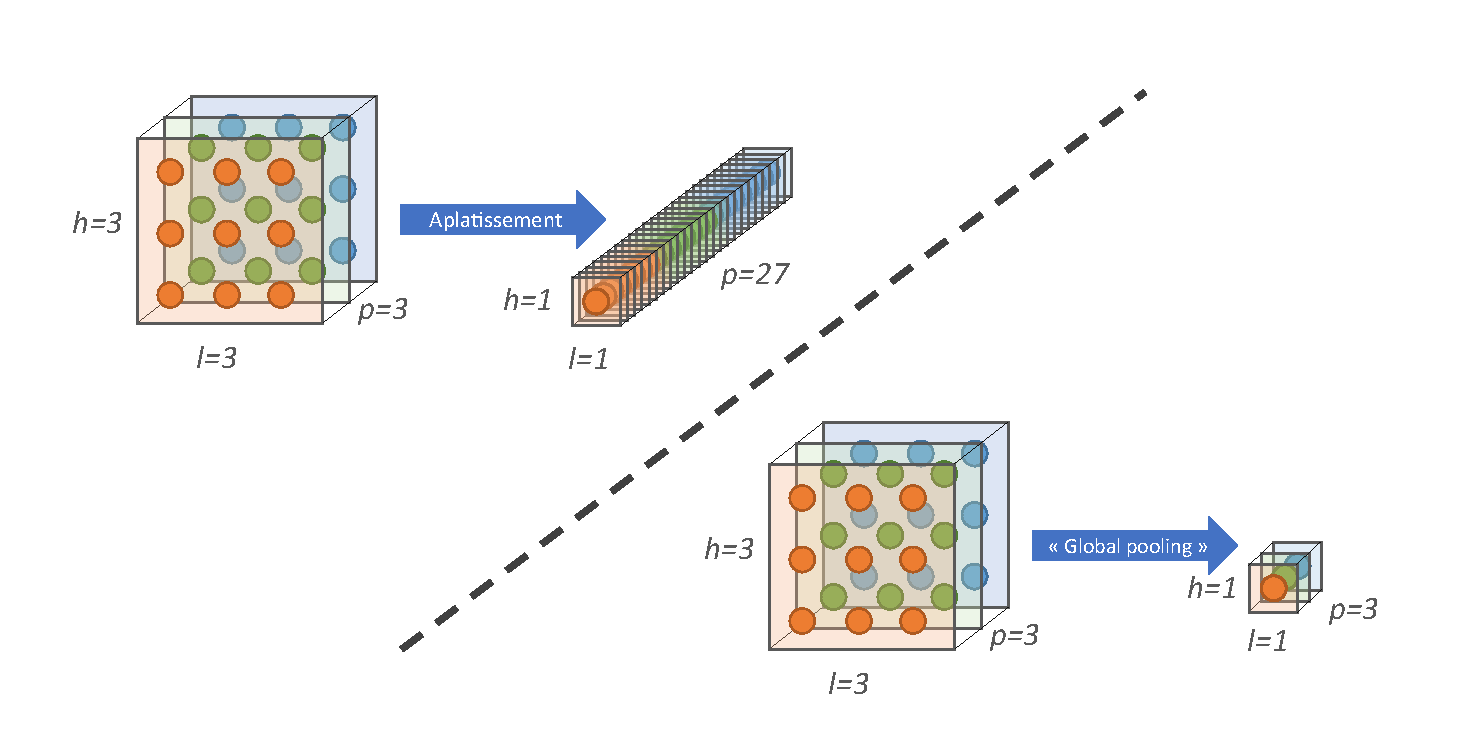
\includegraphics[width=\linewidth]{contents/chapter_5/resources/scheme_global_pooling.pdf}
    \caption{Schéma représentant l'aplatissement et la réduction d'information par \textit{Global Pooling} au sein de \gls{cnn}. Le réseau est entraîné sur des données sources, généralement plus complètes. Puis, les paramètres de la partie liée à l'extraction de caractéristiques sont conservés et réemployés au sein d'une nouvelle problématique cible.}
    \label{fig:scheme_global_pooling}
\end{figure}\par

Bien que la majeure partie des travaux en imagerie médicale s'oriente vers l'architecture Inception-V3, son efficacité n'a pas été formellement démontrée au sein des applications médicales. La raison la plus probable expliquant le choix de cette architecture est la mise à disposition de ses modèles pré-entraînés par la plupart des librairies de \gls{cnn}~\cite{Litjens2017}. Les différentes expériences sur l'apprentissage par transfert se focalisent sur des architectures relativement récentes pré-entraînées sur la base d'image ImageNet et proposées par la bibliothèque \textit{Keras Applications}~\cite{chollet2015a}. Afin de traiter les images dans leur intégralité, ces expérimentations ne considèrent que des réseaux dont les couches d'extraction de caractéristiques sont purement convolutionnelles et donc indépendantes de la taille de l'entrée. Ainsi, sont considérées les architectures de \gls{cnn} représentatives des avancés dans le domaine durant la dernière décennie, dont VGG-16, Inception-V3, ResNet-50 et Inception-ResNet. L'ensemble des réseaux employés et nombre de paramètres extraits associés sont résumés au sein de la \Cref{tab:number_features_transferlearning}. Finalement, la manipulation des \ac{cnn} est réalisée à haut niveau grâce à la bibliothèque logicielle \textit{Keras}~\cite{chollet2015} et est couplée à la bibliothèque de bas niveau \textit{Tensorflow}~\cite{Tensorflow2016}.\par

\begin{table}[H]
    \centering
    \begin{tabular}{lll}
    \toprule
    \textbf{Architecture}               & Global Pooling   & \textbf{Nombre}    \\ \hline
    \multirow{2}{*}{VGG-16}             & Maximum          & 512                \\ \cline{2-3}
                                        & Moyenne          & 512                \\ \hline
    \multirow{2}{*}{Inception-V3}       & Maximum          & 2048               \\ \cline{2-3}
                                        & Moyenne          & 2048               \\ \hline
    \multirow{2}{*}{ResNet-50}          & Maximum          & 2048               \\ \cline{2-3}
                                        & Moyenne          & 2048               \\ \hline
    \multirow{2}{*}{Inception-ResNet}   & Maximum          & 1536               \\ \cline{2-3}
                                        & Moyenne          & 1536               \\
    \bottomrule
    \end{tabular}
    \caption{Liste des architectures de \gls{cnn} employées dans ce chapitre et leur nombre de caractéristiques extraites associées.}
    \label{tab:number_features_transferlearning}
\end{table}\par
\clearpage

\subsection{Analyse préliminaire des méthodes d'extraction}
Cette analyse préliminaire de l'information a pour but de montrer l'impact des méthodes d'extraction de caractéristiques précédemment citées sur le jeu de données mis à disposition. D'une part, cette sous-section propose d'observer l'application des méthodes de transformations précédentes sur deux images typiques de tissus \textbf{malin} et \textbf{bénin}. D'autre part, la capacité de séparation des images de chacune des méthodes précédentes est observée sur l'ensemble des données.\par

Tout d'abord, la présence de motifs plus lisses et moins contrastés au sein des images bénignes peut-être constaté, à l'inverses des motifs présents dans les images malignes. Un exemple de l'application de \gls{glcm} de premier ordre sur des images typiques est visible sur la \Cref{fig:example_glcm}. Il est possible d'observer une uniformité de cette information quelle que soit la direction observée, allant dans le sens de l'utilisation de la moyenne sur les caractéristiques proposées par Haralick et al.~\cite{Wiltgen2008}. Enfin, cette transformation montre une certaine cohérence des transitions dans les images avec des valeurs présentes en majorité sur la diagonale. Néanmoins, ce phénomène semble plus intense sur l'image bénigne, traduisant des transitions plus douces que sur l'image maligne.\par

\begin{figure}[H]
    \centering
    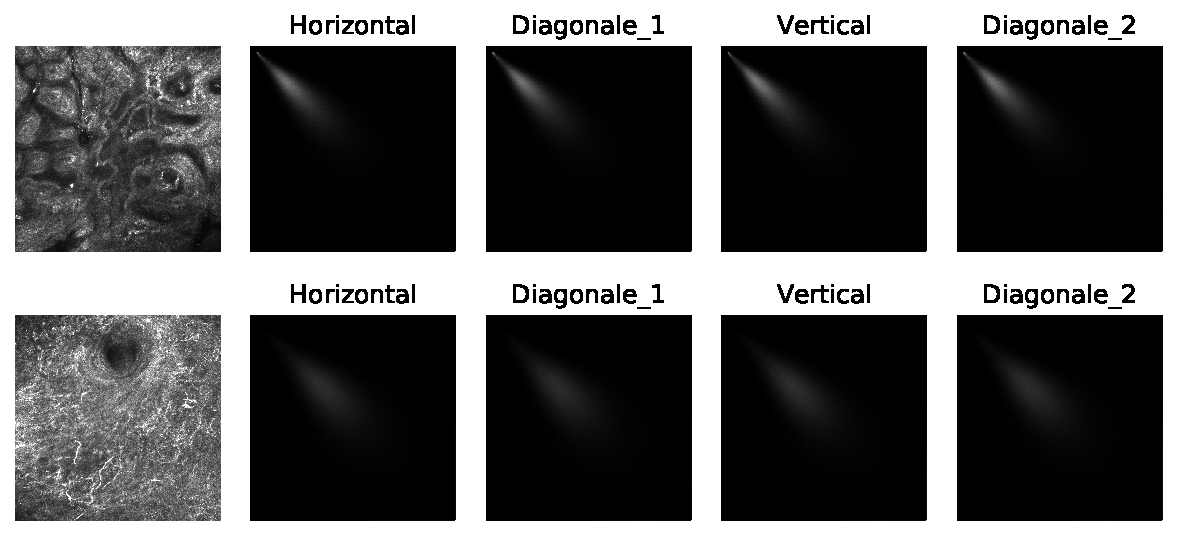
\includegraphics[width=\linewidth]{contents/chapter_5/resources/example_glcm.pdf}
    \caption{Exemple d'extraction de \gls{glcm} de second ordre sur deux images typique. En haut, un cas d'image bénigne ; En bas, une image pathologique typique de \gls{lm}.}
    \label{fig:example_glcm}
\end{figure}\par

La \Cref{fig:example_fft} met en application la transformée de Fourier centrée sur ces deux même images. L'observation du module de cette transformation permet de constater une information plus présente en intensité sur les basses fréquences que sur les hautes fréquences de l'image bénigne, là où sur l'image maligne cette information au centre forme une tâche plus diffuse. En revanche et après une lecture rapide, la direction ne semble pas apporter d'information pertinente comme suggéré par le travail de Wiltgen et al.~\cite{Wiltgen2008}.\par

Enfin, la \Cref{fig:example_wavelet_db4} reflète cette décomposition d'ondelettes de Daubechies tandis que la \Cref{fig:example_wavelet_haar} donne un aperçu de cette même méthode par ondelettes de Haar. L'application de ces transformations permet de constater que les ondelettes de Haar semblent plus propices à isoler les zones de fortes transition que celle de Daubechies. Néanmoins, pour ces deux types d'ondelettes, les décompositions de l'image bénigne semble plus homogène que celle de l'image maligne. De même, l'extraction des hautes fréquences sur l'axe vertical et horizontal semble plus adaptée que l'extraction combinée de ces deux axes pour l'image maligne.\par

\begin{figure}[H]
    \centering
    \includegraphics[width=\linewidth]{contents/chapter_5/resources/example_fft.pdf}
    \caption{Exemple de transformée de Fourier centrée appliquée à deux images typiques, représentation selon le module et la phase. En haut, un cas d'image bénigne ; En bas, une image pathologique typique de \gls{lm}.}
    \label{fig:example_fft}
\end{figure}\par

\begin{figure}[H]
    \centering
    \includegraphics[width=\linewidth]{contents/chapter_5/resources/example_wavelet_db4.pdf}
    \caption{Exemple de transformée en ondelettes de Daubechies appliquée à deux images typiques. En haut, un cas d'image bénigne ; En bas, une image pathologique typique de \gls{lm}.}
    \label{fig:example_wavelet_db4}
\end{figure}\par

\begin{figure}[H]
    \centering
    \includegraphics[width=\linewidth]{contents/chapter_5/resources/example_wavelet_haar.pdf}
    \caption{Exemple de transformée en ondelettes de Haar appliquée à deux images typiques. En haut, un cas d'image bénigne ; En bas, une image pathologique typique de \gls{lm}.}
    \label{fig:example_wavelet_haar}
\end{figure}\par

Dans le but d'évaluer la séparation des classes, l'emploi de la réduction par l'\gls{pca} est privilégié. En effet, les données utilisés dans ce manuscrit contiennent un grand nombre de dimensions et ce malgré l'extraction de caractéristiques, rendant le problème difficile à analyser visuellement. De nombreuses techniques de réduction de l'information permettant une meilleure visualisation sont proposées dans la littérature, comme par exemple le T-SNE~\cite{Maaten2008} mais dont le principal inconvénient réside dans le nombre de degrés de liberté proposés. Néanmoins, l'\gls{pca} est une technique communément acceptée à cette fin~\cite{Himberg2001} et possède l'avantage de ne pas être dépendante de ce type de paramètres. Les informations de variance propre à ces deux axes de projection, ainsi que pour chaque classe leur centre et leur dispersion sur la base de l'écart-type sont proposés pour chaque méthode d'extraction.\par

Ainsi, la \Cref{fig:visualisation_spatial} met en évidence cette technique pour l'ensemble des méthodes spatiales d'extraction. Par ces méthodes, la variance expliquée provenant des deux axes de projection semblent à même de fournir l'intégralité de la variance de ces données. Les caractéristiques extraites à l'aide des techniques d'extraction de premier ordre ne semblent pas suffisante à séparer les diverses classes. En effet, les centres de masses et leur dispersion semblent assez similaires, notamment pour les données bénignes et malignes. De plus, la séparation des classes ne semble pas marquée dans ces divers schémas d'extraction, et les classes bénignes et saines se chevauchent lorsque les méthodes employant les caractéristiques d'Haralick et al. sont utilisées. Par ailleurs, la distribution des méthodes employant ces caractéristiques semble similaire, suscitant de faibles différences entre elles.\par

\begin{figure}[H]
    \centering
    \begin{subfigure}{.49\textwidth}
      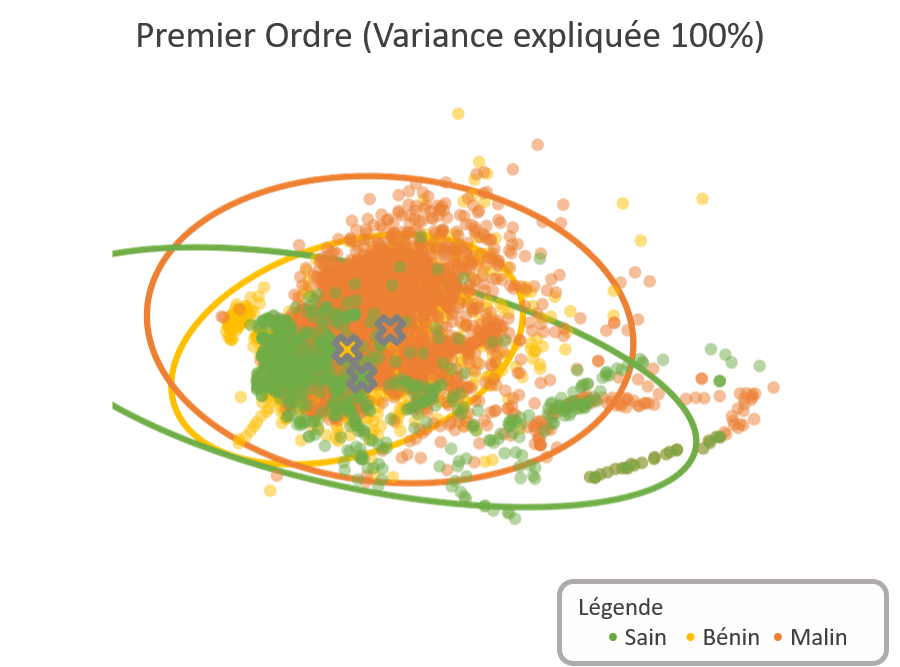
\includegraphics[width=\textwidth]{contents/chapter_5/resources/visualisation_spatial_FirstOrder.png}
    \end{subfigure}
    \begin{subfigure}{.49\textwidth}
      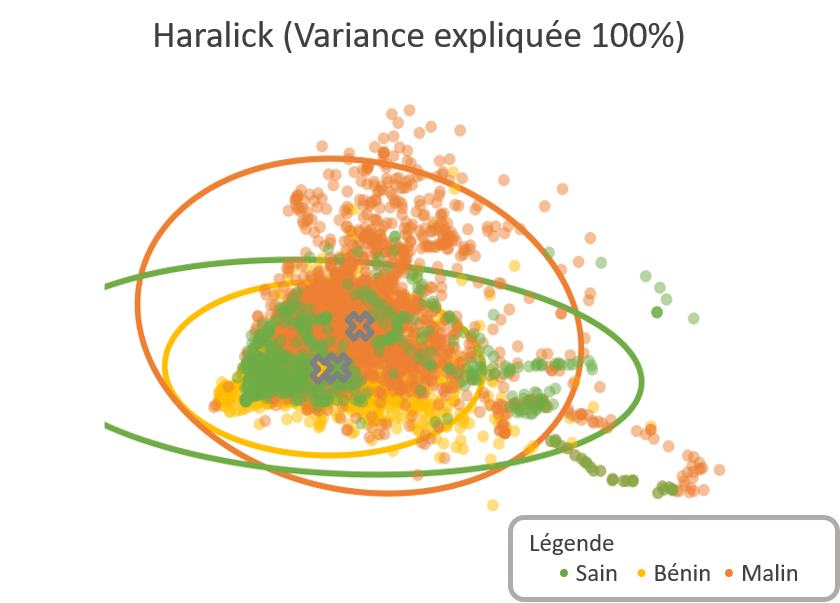
\includegraphics[width=\textwidth]{contents/chapter_5/resources/visualisation_spatial_Haralick.png}
    \end{subfigure}
    
    \begin{subfigure}{.49\textwidth}
      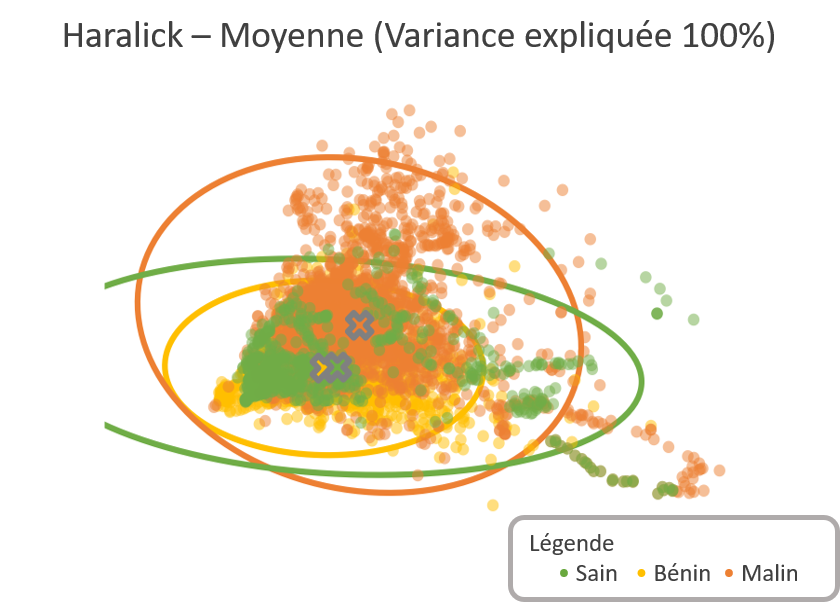
\includegraphics[width=\textwidth]{contents/chapter_5/resources/visualisation_spatial_HaralickMean.png}
    \end{subfigure}
    \begin{subfigure}{.49\textwidth}
      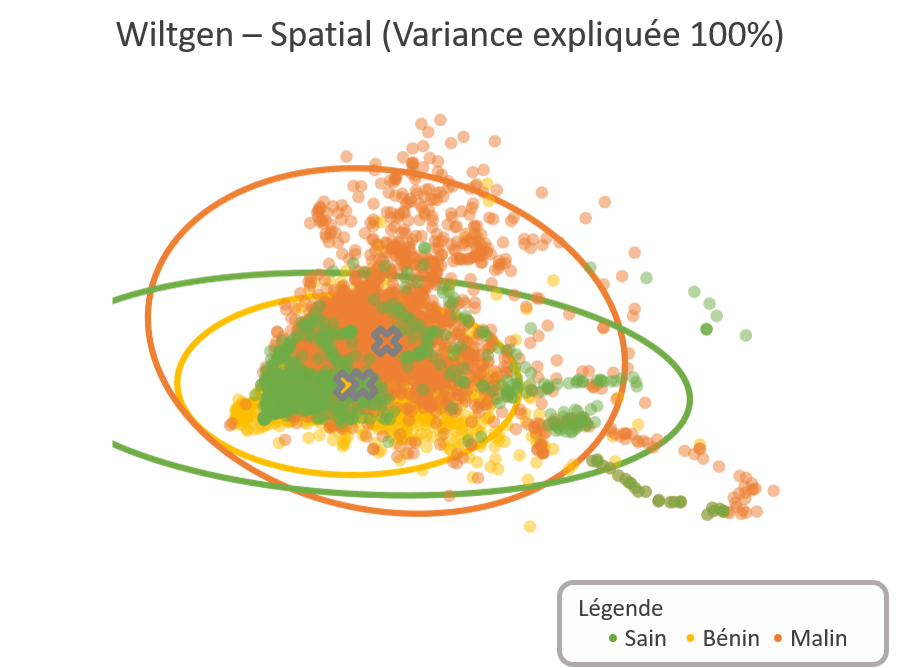
\includegraphics[width=\textwidth]{contents/chapter_5/resources/visualisation_spatial_WiltgenSpatial.png}
    \end{subfigure}
    
    \caption{Visualisation des caractéristiques obtenues par techniques d'extraction spatiales et projection \gls{pca} sur les deux premières composantes.}
    \label{fig:visualisation_spatial}
\end{figure}\par

La \Cref{fig:visualisation_frequency} permet de mettre en évidence la distribution des données extraites par les méthodes d'extraction fréquentielle. Ainsi, les méthodes basées sur l'extraction de caractéristiques de Fourier semblent posséder une distribution similaire quel que soit le nombre de caractéristiques extraites. De plus, la méthode de Fourier proposée par Wiltgen~\cite{Wiltgen2008}, proposant d'extraire des caractéristiques selon diverses directions, ne semble pas influer cette distribution. Du point de vue des méthodes basées sur le principe d'ondelettes, la séparation des données semble être davantage marquée, et l'impact de l'ondelette mère ne semble pas influer sur la distribution des données et des classes. Pour l'ensemble de ces méthodes, les deux premières composantes de l'\gls{pca} semblent suffisantes à exprimer la quasi-intégralité de la variance.\par

Pour finir, la \Cref{fig:visualisation_transfer} recense les projections par \gls{pca} de l'ensemble des méthodes d'extraction basée sur des architecture de \gls{cnn} pré-entraînées, catégorisées sous le terme de transfert par apprentissage. Une différence notable est à remarquer entre les architectures utilisant une couche de \textit{Global Pooling - Moyen} et celle utilisant une couche de \textit{Global Pooling - Maximum}. En effet, la séparation entre classes est marquée de manière plus importante lorsque qu'une couche de \textit{Global Pooling - Moyen} est employée. De plus, cette séparation semble être plus prononcée sur les architectures Inception-V3 et ResNet-50, Enfin, par ces méthodes la variance exprimée sur les deux premières composantes n'est que de 20\% à 40\%. Ce dernier constat s'explique par la grande quantité d'informations initialement proposée par ces architectures, soit entre 512 et 2048 caractéristiques extraites en comparaison d'une ou quelques dizaines pour les méthodes manuelles.\par

\begin{figure}[p]
    \centering
    \begin{subfigure}{.49\textwidth}
      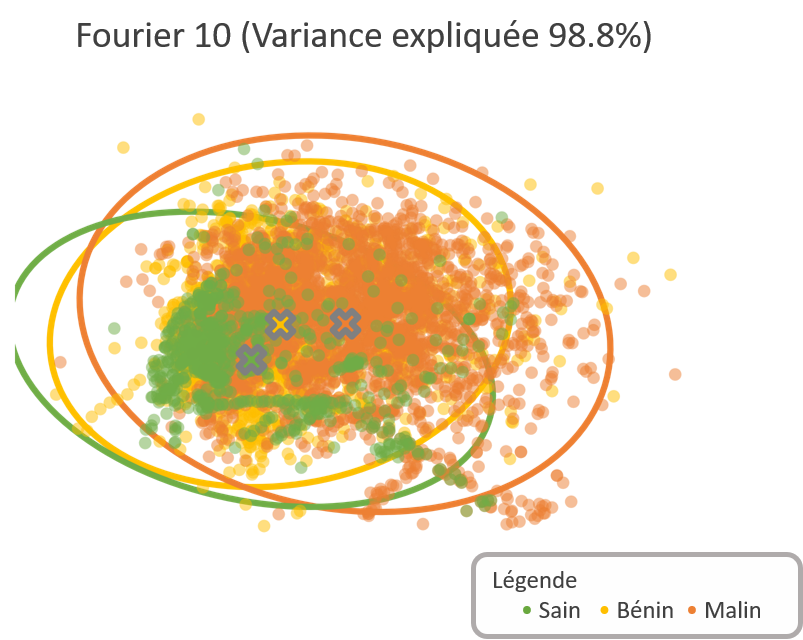
\includegraphics[width=\textwidth]{contents/chapter_5/resources/visualisation_frequency_Fourier10.png}
    \end{subfigure}
    \begin{subfigure}{.49\textwidth}
      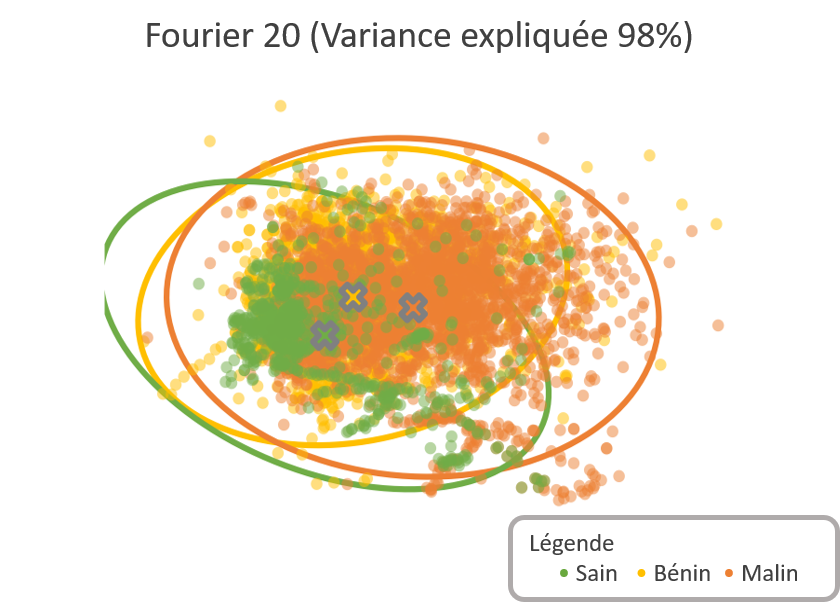
\includegraphics[width=\textwidth]{contents/chapter_5/resources/visualisation_frequency_Fourier20.png}
    \end{subfigure}
    
    \begin{subfigure}{.49\textwidth}
      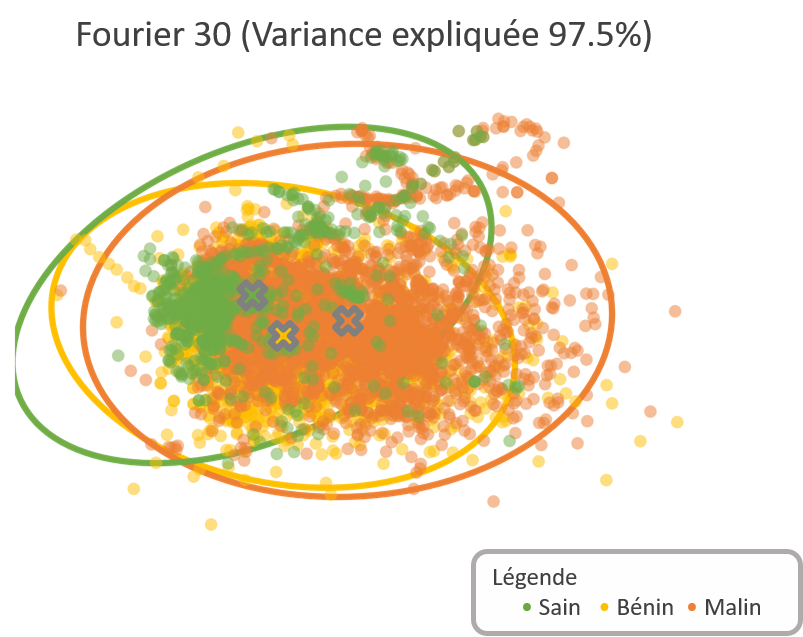
\includegraphics[width=\textwidth]{contents/chapter_5/resources/visualisation_frequency_Fourier30.png}
    \end{subfigure}
    \begin{subfigure}{.49\textwidth}
      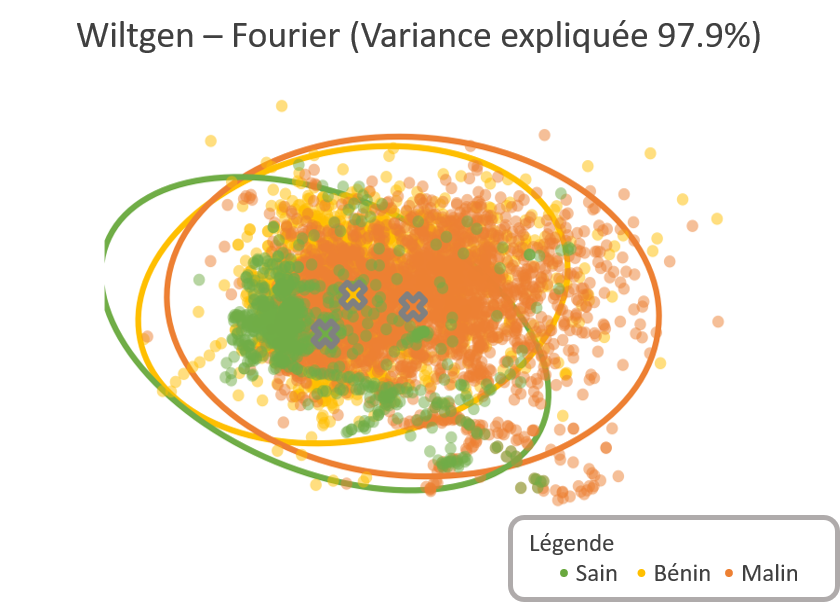
\includegraphics[width=\textwidth]{contents/chapter_5/resources/visualisation_frequency_WiltgenFourier.png}
    \end{subfigure}
    
    \begin{subfigure}{.49\textwidth}
      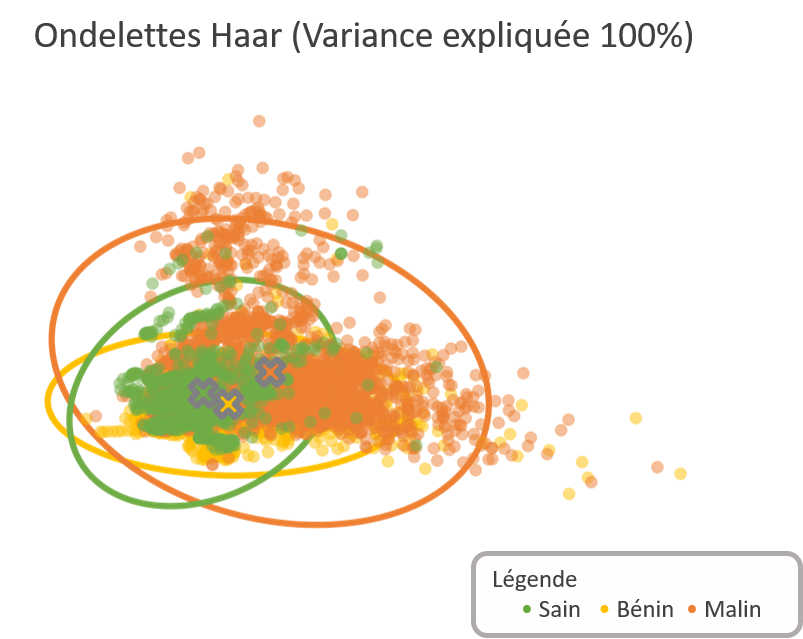
\includegraphics[width=\textwidth]{contents/chapter_5/resources/visualisation_frequency_Haar.png}
    \end{subfigure}    
    \begin{subfigure}{.49\textwidth}
      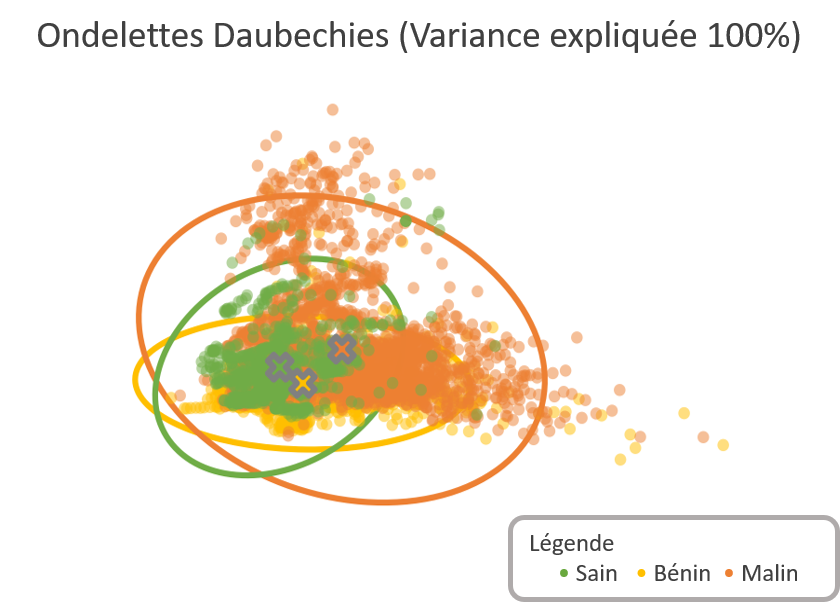
\includegraphics[width=\textwidth]{contents/chapter_5/resources/visualisation_frequency_Daubechies.png}
    \end{subfigure}
    
    \caption{Visualisation des caractéristiques obtenues par techniques d'extraction fréquentielles et projection \gls{pca} sur les deux premières composantes.}
    \label{fig:visualisation_frequency}
\end{figure}\par

\begin{figure}[p]
    \centering
    \begin{subfigure}{.49\textwidth}
      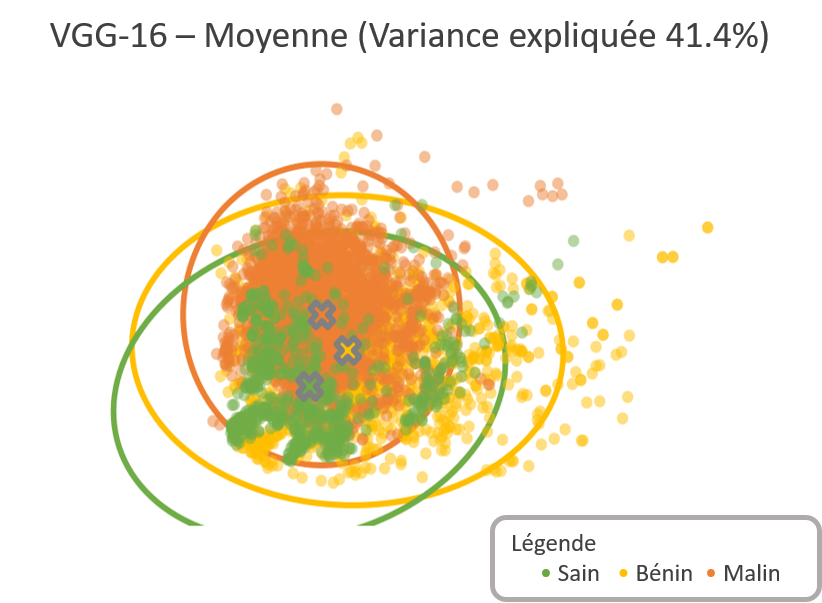
\includegraphics[width=\textwidth]{contents/chapter_5/resources/visualisation_transfer_VGG16Avg.png}
    \end{subfigure}
    \begin{subfigure}{.49\textwidth}
      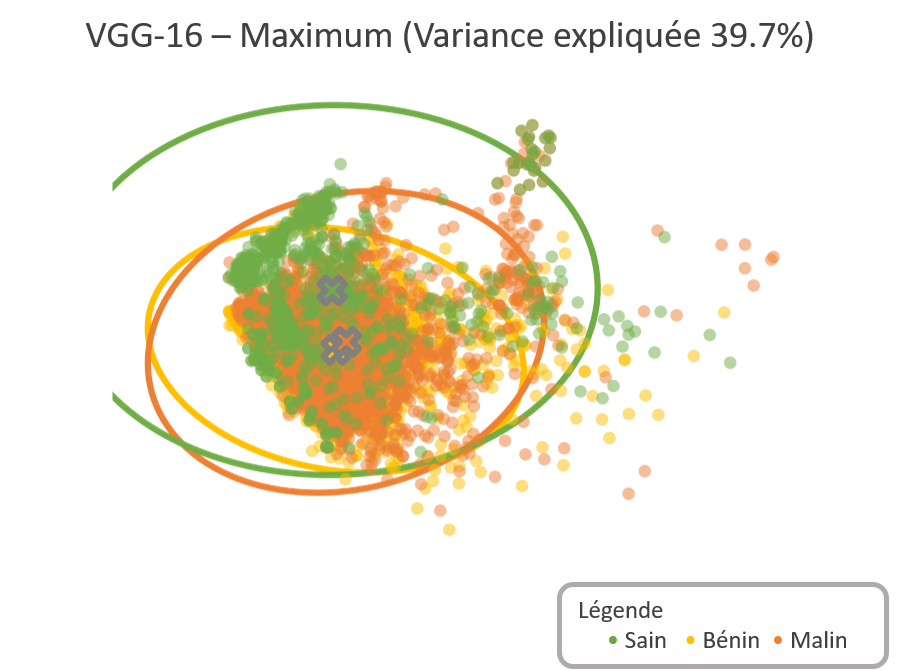
\includegraphics[width=\textwidth]{contents/chapter_5/resources/visualisation_transfer_VGG16Max.png}
    \end{subfigure}
    
    \begin{subfigure}{.49\textwidth}
      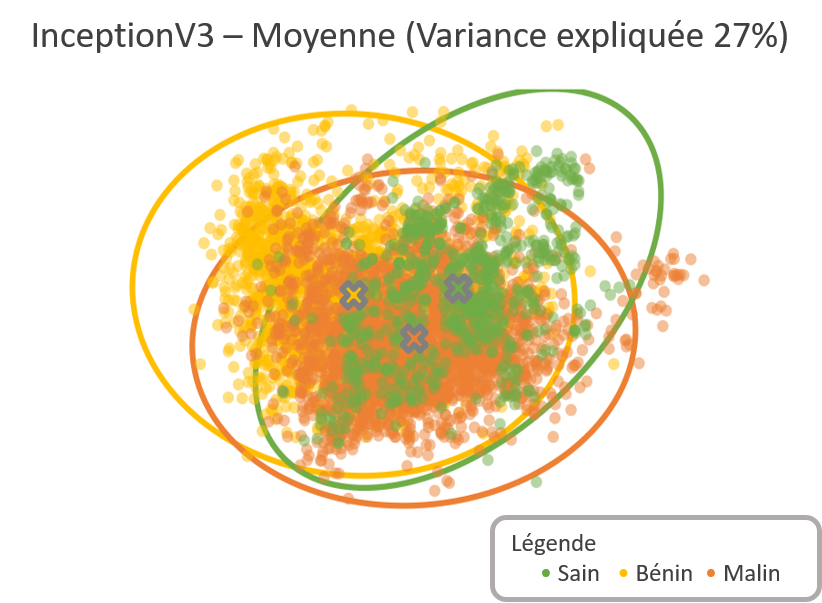
\includegraphics[width=\textwidth]{contents/chapter_5/resources/visualisation_transfer_InceptionV3Avg.png}
    \end{subfigure}
    \begin{subfigure}{.49\textwidth}
      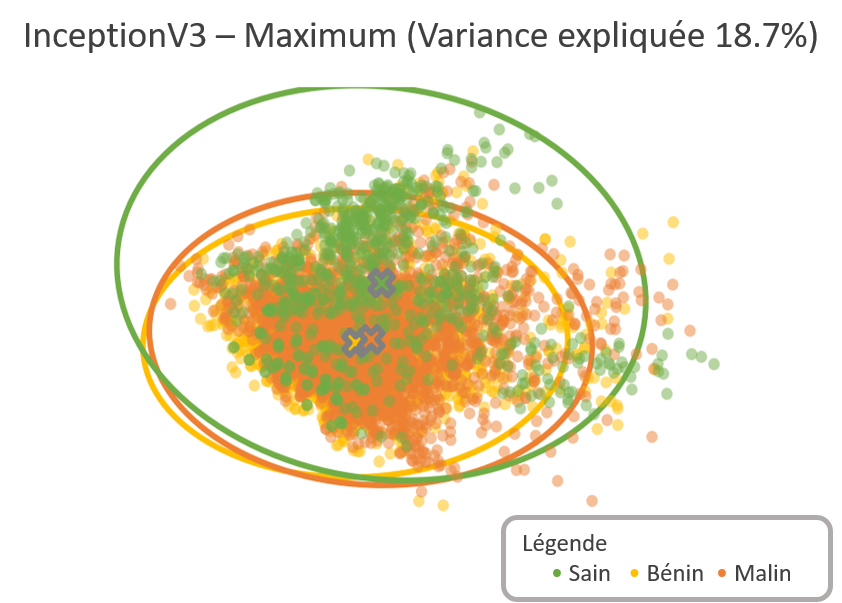
\includegraphics[width=\textwidth]{contents/chapter_5/resources/visualisation_transfer_InceptionV3Max.png}
    \end{subfigure}
    
    \begin{subfigure}{.49\textwidth}
      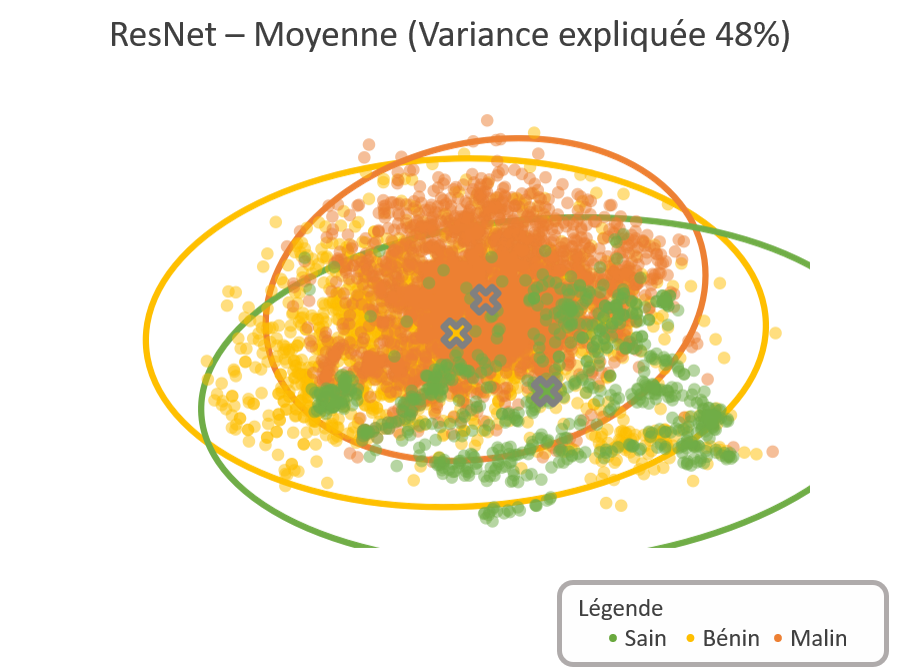
\includegraphics[width=\textwidth]{contents/chapter_5/resources/visualisation_transfer_ResNetAvg.png}
    \end{subfigure}
    \begin{subfigure}{.49\textwidth}
      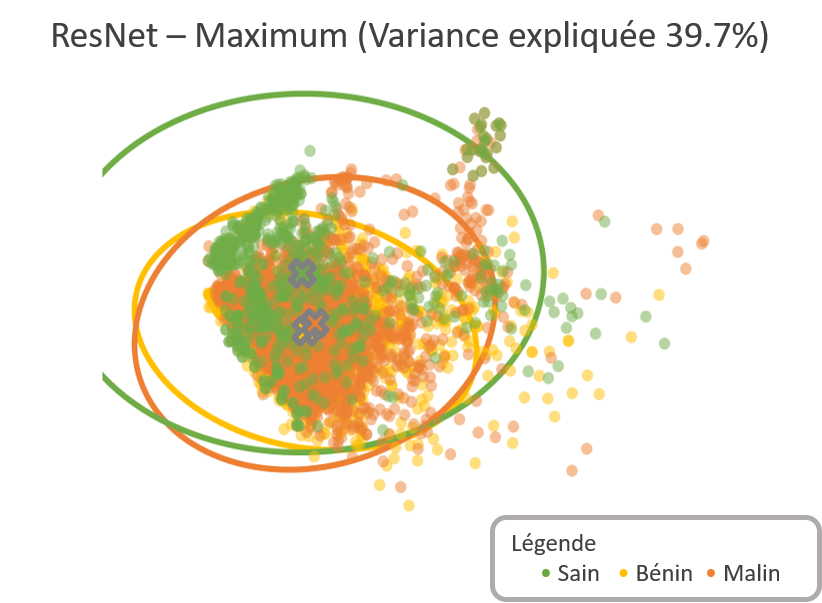
\includegraphics[width=\textwidth]{contents/chapter_5/resources/visualisation_transfer_ResNetMax.png}
    \end{subfigure}
    
    \begin{subfigure}{.49\textwidth}
      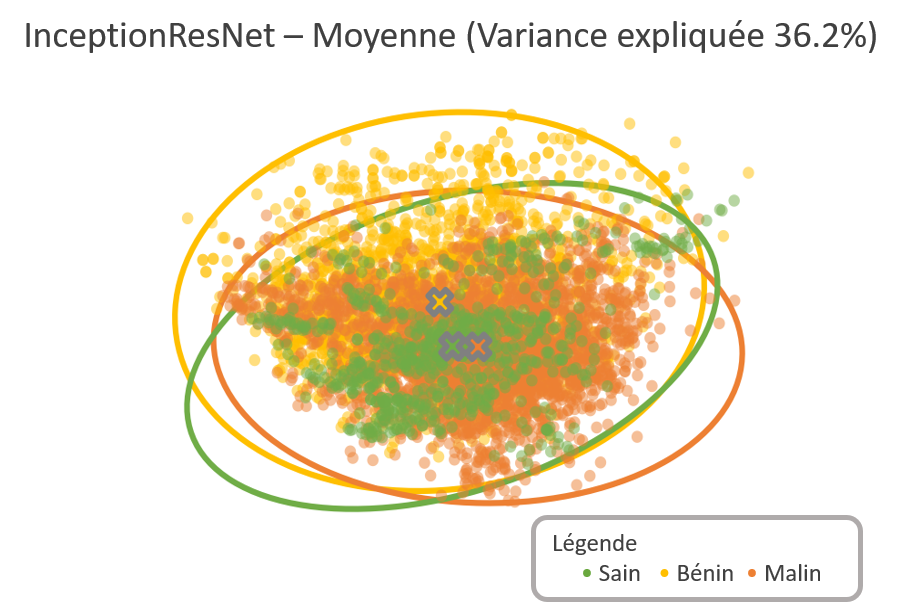
\includegraphics[width=\textwidth]{contents/chapter_5/resources/visualisation_transfer_InceptionResNetAvg.png}
    \end{subfigure}
    \begin{subfigure}{.45\textwidth}
      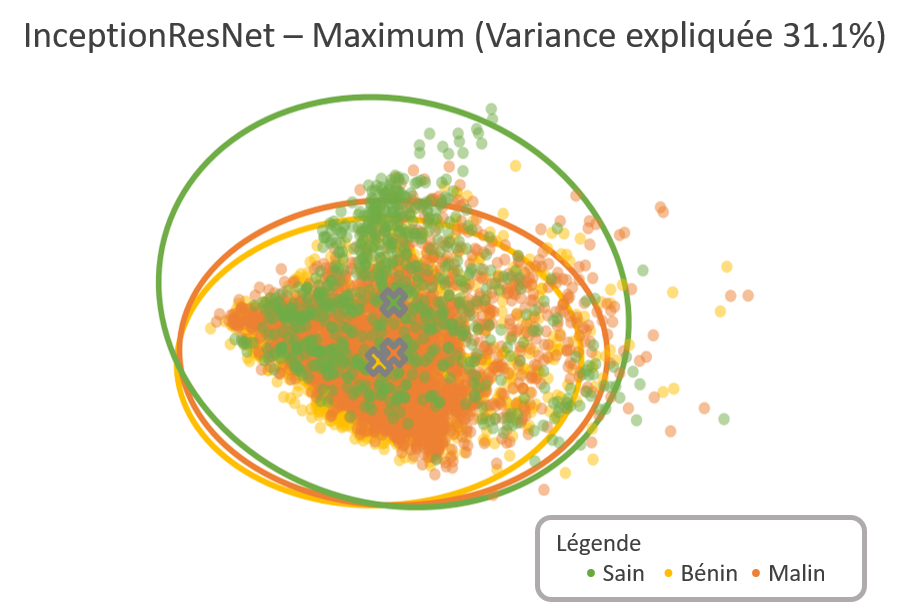
\includegraphics[width=\textwidth]{contents/chapter_5/resources/visualisation_transfer_InceptionResNetMax.png}
    \end{subfigure}
    
    \caption{Visualisation des caractéristiques obtenues par techniques d'extraction basées sur des réseaux de type \gls{cnn} pré-entraînés sur la base ImageNet et projection \gls{pca} sur les deux premières composantes.}
    \label{fig:visualisation_transfer}
\end{figure}\par

\clearpage


%%%%%%%%%%%%%%%%%%%%%%%%%%%%%%%%%% 
%%%%%%%%%%%%%%%%% PRE TRAITEMENTS
\section{Pré-traitements de caractéristiques}
Cette partie dédiée au pré-traitement de caractéristiques, se consacre à l'ensemble des transformations opérées après extraction de l'information par le biais des techniques évoquées en \Cref{chap:feature_extraction}. Au sein de cette section sont abordées les diverses solutions pouvant parfaire la classification des images \gls{rcm}. En effet, de nombreuses contraintes peuvent affecter le bon déroulement de la classification~:
\begin{itemize}
    \item un \textbf{déséquilibre des annotations} des divers types de tissus a séparé bien que celui-ci ait été minimisée,
    \item un \textbf{nombre de caractéristiques} trop important conduisant à du sur-apprentissage ou à des difficultés à séparer le problème (voir l'extraction de caractéristiques par \gls{cnn}),
    \item ou encore \textbf{une information non consistante}.
\end{itemize}\par

Ainsi, cette partie tente de répondre à ces questions à l'aide de différents domaines d'étude visant à corriger tout ou partie de ces éléments. Ces solutions sont abordées d'un point de vue logique en termes de processus de classification. Dans un premier temps, la \textbf{normalisation} des caractéristiques est présentées ainsi que son intérêt au sein de processus de classification. Dans un second temps, les méthodes de \textbf{réduction de l'information} sont proposées dans le cadre de l'extraction de caractéristiques par \gls{cnn} afin de limiter la quantité de ces dernières. Finalement, le \textbf{balancement de données} et ses principales stratégies sont mises à disposition du lecteur.

\subsection{Réduction de dimensions}
Dans le domaine de l'apprentissage automatique, la réduction de dimensions est une technique qui permet de diminuer le nombre de dimensions afin de rendre un problème moins complexe, tout en conservant une information suffisante à la résolution du problème. Également, elle est un moyen de se prévenir du «Fléau de la dimension», phénomène qui met en perspective d'une part la croissance exponentielle de l'ajout de nouvelles dimensions à la dilution des divers échantillons dans cet espace. Ce dilemme a pour principales conséquences d'augmenter la complexité d'un problème, la durée nécessaire à sa résolution mais également d'engendrer des risques de sur-apprentissage.\par

Les caractéristiques extraites par méthode spatiales et fréquentielles étant assez restreintes (respectivement de 14 à 56 variables et, de 10 à 39 variables), l'impact de la réduction de dimension n'est pas étudié sur ces méthodes. En revanche, le nombre des caractéristiques extraites par méthode de transfert de connaissance est suffisamment important (entre 512 et 2048 variables) pour justifier de l'utilisation de cette réduction et d'étudier leur impact sur ces cas particuliers.\par

A cette fin, deux catégories de méthodes cohabitent~: d'une part les méthodes de sélection de caractéristiques qui réduisent l'espace en décimant certaines dimensions jugées non pertinentes à la résolution du problème ; d'autre part les méthodes par projection ou transformation de l'espace existant qui réduisent et modifient les valeurs existantes. Dans la mesure où ces techniques s'appliquent sur les méthodes d'extraction par transfert de connaissances, cette investigation ne porte que sur cette seconde catégorie de méthodes. En effet, les méthodes par sélection de caractéristiques ne semblent pas pertinentes dans le cadre de caractéristiques auto-déterminées par des réseaux profonds.\par

L'\gls{pca} est l'une de ces techniques, dont l'idée majeure est de retirer l'information redondante pour ne conserver que l'information de variance, supposée contenir l'information. Cette méthode cherche ainsi à identifier les axes selon lesquels la variation des données est maximisée. Il sera ensuite nécessaire de déterminer un nombre d'axes suffisant à séparer le problème (réduction du nombre de caractéristiques). Ainsi, ce travail retient les seuils de la littérature les plus pertinents de cette variance cumulée, à savoir des valeurs de 95\%, 97,5\% et 99\%.\par

L'\gls{lda} est une seconde technique employée à une fin de réduction de l'information, pour laquelle sont recherchés des axes de projection qui maximisent la variance inter-groupe. Pour comparaison, la variance est le résultat de la somme de la variance intra-groupe et inter-groupe. De manière similaire à la précédente technique, sont retenus des seuils de variance cumulée de 95\%, 97,5\% et 99\%.\par

La \Cref{tab:summary_reduction_methods} reprend ces diverses méthodes ainsi que leurs paramètres mis en oeuvre conjointement à l'utilisation des méthodes d'extraction de caractéristiques sur base de transfert de connaissances.\par 

\begin{table}[H]
    \centering
    \begin{tabular}{lll}
        \toprule
        \textbf{Méthode}       & \textbf{Paramètre}                 & \textbf{Valeurs}                      \\ \midrule
        \gls{pca}              & \multirow{2}{*}{Variance expliquée}& \multirow{2}{*}{[95\%, 97,5\%, 99\%]} \\ \cline{1-1}
        \gls{lda}              &                                    &                                       \\ 
        \bottomrule
    \end{tabular}
    \caption{Liste des méthodes de réduction employées et leurs paramètres associés.}
    \label{tab:summary_reduction_methods}
\end{table}\par

\subsection{Normalisation de caractéristiques}
\label{subsec:features_normalisation}
Selon le domaine d'étude visée, la normalisation de caractéristiques peut être l'une des étapes cruciales quant au bon déroulement de ce processus de classification. Cette recherche a été amenée à considérer cet aspect suite à la dégradation de résultats au sein d'un travail proche de la thématique de ce manuscrit portant sur la classification d'images de dermatoscopie~\cite{Celebi2007}.\par

Il est communément admis que des méthodes tels que les \gls{knn} dont le principe repose sur des critères de distance, peuvent être fortement affectées par des caractéristiques non normalisées. Pour d'autres méthodes de classification, cette normalisation des caractéristiques fait davantage appel à un bon sens vis-à-vis de leur principe de fonctionnement. Certains travaux mettent en évidence la dégradation des performances sur les \gls{svm}~\cite{Juszczak2002} mais également les réseaux de neurones~\cite{Celebi2007}.\par

Diverses méthodes ont ainsi été proposées afin de remédier à ces défauts de distribution de l'information. L'un de ces travaux propose de réduire l'erreur de classification de modèles \gls{svm} par l'apport de normalisations tenant compte de la variance, du maximum ou encore conjointement du minimum et du maximum~\cite{Juszczak2002}. Le travail mené par Celebi et al.~\cite{Celebi2007} propose une normalisation des caractéristiques à l'aide de la \textit{Cote Z} ou \textit{Standard score}, c’est-à-dire par soustraction de la moyenne au sein d'un même groupe de caractéristiques puis par division de l'écart-type de ce même groupe.\par

Afin de couvrir au mieux cette problématique de normalisation, deux des méthodes majeures de la littérature sont envisagées pour la suite de cette sous-section, dont l'\Cref{eq:scaling_methods} reprend les expressions sous forme mathématique. Ainsi, sont considérées~:
\begin{itemize}
    \item la normalisation par \textit{Mininimum / Maximum}~\cite{Juszczak2002},
    \item et la normalisation \textit{Standard}~\cite{Celebi2007}.
\end{itemize}\par

\begin{equation} 
    \label{eq:scaling_methods}
    \begin{split}
    Minimum/Maximum&=\frac{X-min(X)}{max(X)-min(X)}  \\
    Standard&=\frac{X-\mu{}}{\sigma}	    
    \end{split}
\end{equation}

\subsection{Balancement de données}
\label{subsec:balancement}
L'une des problématiques associées de manière récurrente à l'apprentissage sur des données réelles est celle de la répartition homogène des annotations, en opposition aux domaines impliquant des données synthétiques pouvant provenir de modèles génératifs par exemple. Ces déséquilibres d'annotations sont qualifiés sous le terme anglophone de \textit{class imbalance}~\cite{Prati2009, He2009}.\par

Ces déséquilibres sont propres à de nombreux domaines d'applications, mais touchent essentiellement des champs d'activités dans lesquels la tâche visée correspond à la détection d'événements isolés au sein d'une population, comme par exemple~: 
\begin{inlinerate}
    \item les comportements déviants (fraude bancaire~\cite{Phua2004}),
    \item le respect de critère de qualité (vérification de pièces industrielles~\cite{Wu2018}),
    \item ou encore d'anormalités cliniques (cancers ou autres pathologies cliniques~\cite{Celebi2007}).
\end{inlinerate}\par

Certains choix peuvent permettre de limiter l'impact d'un déséquilibre d'annotations. Ainsi, la sélection d'une métrique adéquate peut permettre de limiter la dépendance au données~: la substitution de la précision par des mesures telles que l'\gls{auc}~\cite{Celebi2007} ou le \fscore{} sont des solutions pertinentes dans de telles situations. Néanmoins, la plupart des modèles de classification échouent à classifier convenablement les données dans des situations de forts déséquilibres. Ces modèles préfèrent prédire constamment la classe majoritaire, pour minimiser le coût de l'erreur~\cite{Huang2013}. Dans le cadre de modèles basés sur des arbres de décision, la stratégie générale propose de déterminer les critères majeurs de séparation par partitionnement successif des données. Ce partitionnement conduit inéluctablement à un affaiblissement des classes minoritaires~\cite{He2009}. Deux catégories d'approches coexistent pour solutionner ces déséquilibres~\cite{Huang2013}, d'une part les approches par augmentation ou décimations des diverses catégories d'annotation, et d'autres part les approches algorithmiques qui consistent à pondérer la valeur des annotations afin de prendre en considération le déséquilibre de l'information~\cite{Ting2002,He2009,Thai2010}.\par

En premier lieu, ces déséquilibres de classes peuvent être corrigés par des méthodes simples permettant de pallier ces défauts~\cite{Prati2009, He2009}. Une première catégorie de ces méthodes consiste à \textbf{sous-échantillonner} les données jusqu'à obtenir une égalité entre les classes. Son principe le plus simple est celui du \textbf{sous-échantillonnage aléatoire} consistant à décimer de manière aléatoire les données des classes majoritaires afin d'égaler les échantillons de la classe minoritaire. A l'inverse, une autre catégorie consiste à \textbf{sur-échantillonner} les données possédées afin d'obtenir à nouveau une égalité entre classes. Le principe le plus simple est celui du \textbf{sur-échantillonnage aléatoire} consistant à dupliquer aléatoirement les échantillons des classes minoritaires afin d'égaler le nombre d'éléments de la classe majoritaire. Le schéma en \Cref{fig:scheme_data_balancing} reprendre l'idée de ces deux principes.\par

En second lieu, des approches par correction des données plus avancées ont été proposées dans la littérature afin de compléter les méthode de sur-échantillonage et sous-échantillonage. L'un des exemples majeurs de ces méthodes de sur-échantillonage est la méthode \gls{smote}~\cite{Chawla2002}, dont le principe permet de générer par interpolation de nouvelles instances en choisissant aléatoirement une première instance \textit{a} et de prendre aléatoirement parmi ses plus proches voisins une seconde instance \textit{b}. En ce qui concerne les méthode de sous-échantillonage, peuvent être citées la méthode \gls{tl}~\cite{Tomek1976} et \gls{enn}~\cite{Wilson1972} utilisées pour enlever les incohérences au sein des données. Néanmoins, ces méthodes seules possèdent diverses lacunes et sont solutionnées à l'aide de nouvelles approches qualifiées d'\textit{hybrides} mêlant ces deux aspects. Parmi cette nouvelle catégorie, ce travail considère l'approche \textbf{\gls{smote} + \gls{tl}} et l'approche \textbf{\gls{smote} + \gls{enn}} dont les principes consistent à synthétiquement augmenter les données par la méthode \gls{smote}, puis à nettoyer les données constituées d'instances réelles et synthétiques par la méthode \gls{tl} ou \gls{enn}.

\begin{figure}[H]
    \centering
    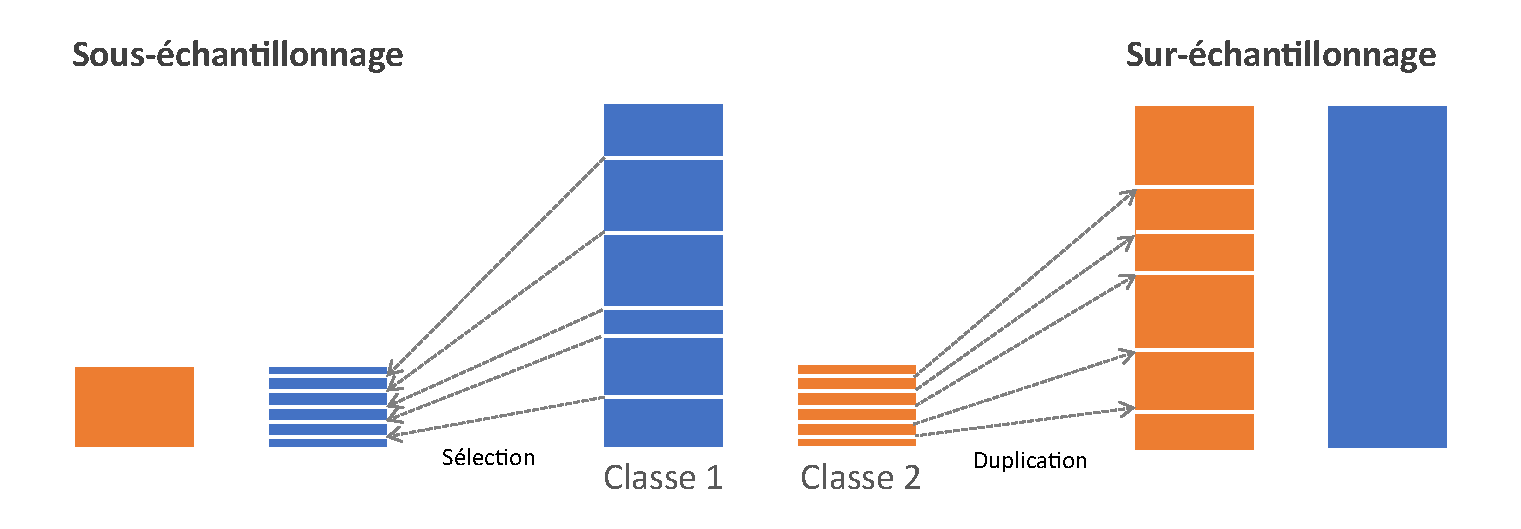
\includegraphics[width=\linewidth]{contents/chapter_5/resources/scheme_data_balancing.pdf}
    \caption{Schéma des deux stratégies principales de balancement de données. A gauche, la stratégie de sous-échantillonnage, dans laquelle des éléments sont aléatoirement choisis jusqu'à réduire l'ensemble des classes au nombre d'éléments de la classe minoritaire ; A droite, la stratégie de sur-échantillonnage, dans laquelle les éléments des classes minoritaires sont dupliqués aléatoirement. }
    \label{fig:scheme_data_balancing}
\end{figure}\par

En opposition à ces méthodes dédiées, \textbf{les approches par pondération} des échantillons consistent à gérer le déséquilibre des annotations en appliquant des poids d'importance différente selon la provenance de l'échantillon lors de l'apprentissage du modèle. Cette approche par défaut est privilégiée puisqu'elle permet de contrer de manière assez intuitive ces déséquilibres.\par

Dans l'optique de récapituler cette partie, les méthodes utilisées dans le but de corriger le déséquilibre des données sont référencée dans la \Cref{tab:summary_balancement_methods}. Afin de traiter au mieux cette tâche, le balancement de données par les différentes stratégies évoquées est réalisé avec l'aide de la librairie logicielle \textit{Imbalanced-learn}~\cite{Lemaitre2017}. La correction par pondération est réalisée avec l'aide de la bibliothèque logicielle \textit{Scikit-learn}~\cite{pedregosa2011}.\par

\begin{table}[H]
    \centering
    \begin{tabular}{ll}
        \toprule
        \textbf{Catégorie}                  & \textbf{Méthode}          \\ \hline
        Sous-échantillonnage                & Aléatoire                 \\ \hline
        Sur-échantillonnage                 & Aléatoire                 \\ \hline
        \multirow{2}{*}{Hybride}            & \gls{smote} + \gls{tl}    \\ \cline{2-2}
                                            & \gls{smote} + \gls{enn}   \\ \bottomrule
    \end{tabular}
    \caption{Liste des diverses méthodes de balancement mises en œuvre pour corriger les déséquilibre de données.}
    \label{tab:summary_balancement_methods}
\end{table}\par

\section{Processus de prédiction}
Cette section dédiée au processus de prédiction se consacre à la dernière étape de traitement des données au sein du processus de classification supervisé. D'une part, son objectif est de présenter les divers modèles de classification utilisés pour la séparation de l'information. D'autre part, son objectif est de mettre en exergue le processus d'évaluation et les raisons ayant justifié ces choix.\par

\subsection{Méthodes de prédiction}
Afin d'œuvrer à la séparation des échantillons en notre possession sur la base de leurs caractéristiques, divers modèles de classification sont sollicités et pour lesquels les performances sont évaluées. En effet, bien que les avantages et inconvénients de la plupart d'entre eux aient été évoqués au sein de la \Cref{sec:models_settings}, seules les performances de classification mesurées sur le jeu de données de référence sont retenues.\par

\begin{table}[H]
    \centering
    \begin{tabular}{cll}
        \toprule
        \textbf{Modèle}                                 & \textbf{Hyperparamètre}   & \textbf{Valeurs}                          \\ \midrule
        \multirow{4}{*}{\gls{cart}}                     & Profondeur maximum        & [3, $\infty$]                             \\ \cmidrule{2-3} 
                                                        & Critère de qualité        & [Gini, Entropie]                          \\ \cmidrule{2-3}   
                                                        & Caractéristiques maximum  & [1, 2, 3, 4, 5, 6, 7, 8, 9]               \\ \cmidrule{2-3}   
                                                        & Échantillons minimum      & [1, 2, 3, 4, 5, 6, 7, 8, 9]               \\ \midrule 
        \multirow{4}{*}{\gls{rf}}                       & Profondeur maximum        & [3, $\infty$]                             \\ \cmidrule{2-3} 
                                                        & Critère de qualité        & [Gini, Entropie]                          \\ \cmidrule{2-3}   
                                                        & Caractéristiques maximum  & [1, 2, 3, 4, 5, 6, 7, 8, 9]               \\ \cmidrule{2-3}   
                                                        & Échantillons minimum      & [1, 2, 3, 4, 5, 6, 7, 8, 9]               \\ \midrule 
        \multirow{4}{*}{\gls{gb}}                       & Profondeur maximum        & [3, $\infty$]                             \\ \cmidrule{2-3}
                                                        & Critère                   & [MSE, MAE]                                \\ \cmidrule{2-3} 
                                                        & Caractéristiques maximum  & [1, 2, 3, 4, 5, 6, 7, 8, 9]               \\ \cmidrule{2-3}   
                                                        & Échantillons minimum      & [1, 2, 3, 4, 5, 6, 7, 8, 9]               \\ \midrule 
        \gls{svm} - Noyau linéaire                      & C                         & [0,001, 0,01, 0,1, 1, 10, 100, 1000]      \\ \midrule
        \multirow{2}{*}{\gls{svm} - Noyau RBF}          & C                         & [0,001, 0,01, 0,1, 1, 10, 100, 1000]      \\ \cmidrule{2-3}   
                                                        & Gamma                     & [0,001, 0,01, 0,1, 1, 10, 100, 1000]      \\ \midrule 
        \multirow{5}{*}{\gls{mlp}}                      & Couche cachées            & [(20,), (20,20,), (20,20,20,)]            \\ \cmidrule{2-3}
                                                        & Activation                & [Tanh, ReLu]                              \\ \cmidrule{2-3}
                                                        & Solveur                   & [SGD, Adam]                               \\ \cmidrule{2-3}
                                                        & Alpha                     & [0,001, 0,01, 0,1, 1, 10, 100, 1000]      \\ \cmidrule{2-3}
                                                        & Taux d'apprentissage      & [Constant, Adaptatif]                     \\ \bottomrule 
    \end{tabular} 
    \caption{Table recensant l'ensemble des modèles de classification et leurs hyperparamètres évalués lors des expériences de ce travail.}
    \label{tab:image_classification_models_hyperparameters}
\end{table}\par

Dans un premier temps, le modèle \textbf{\gls{cart}} est utilisé afin de réaliser la séparation des données, son choix étant motivé par l'un des travaux dont la thématique est similaire à celle de ce travail~\cite{Wiltgen2008}. Néanmoins, ces modèles tendent au sur-apprentissage dans des contextes où les dimensions sont nombreuses, ainsi sont utilisées de manière complémentaires les modèles \textbf{\gls{rf}}~\cite{Breiman2001} et \textbf{\gls{gb}} plus aptes à gérer cet aspect. Dans un second temps, les modèles \textbf{\gls{svm}} à noyaux \textit{linéaires} et à \textit{base radiale} sont employés pour cette même tâche de séparation des données, et sont motivés par leur utilisation dans de nombreux contextes de classification pour lesquels ils ont été démontrés comme robustes~\cite{Smach2008a}. Ces modèles sont également employés dans des contextes de classification de lésion de la peau~\cite{Celebi2007}. Enfin, la piste des \textbf{\gls{mlp}} est envisagée afin d'envisager cette problématique de manière non linéaire.\par

Afin d'obtenir les meilleurs performances sur ces modèles, les hyperparamètres associés à chacun d'entre eux sont affinés en respectant la procédure de la prochaine sous-section. Néanmoins, un compromis entre le temps d'exécution et le nombre de ces valeurs est nécessaire, conduisant ce travail à opter pour celles les plus couramment utilisées. L'ensemble des modèles de classification mais également leurs hyperparamètres et leurs valeurs associés sont recensés dans la \Cref{tab:image_classification_models_hyperparameters}. Par ailleurs, les modèles de classification employés par ce travail proviennent de la bibliothèque logicielle \textit{Scikit-learn}~\cite{pedregosa2011}.\par

\subsection{Procédure d'évaluation}
Pour réaliser l'évaluation, est employée une validation croisée imbriquée déjà discutée dans le \Cref{sec:models_settings}. Cette structure de validation est choisie car moins sujet au biais~\cite{Cawley2010}, de plus une valeur de $k$ comprise entre 5 et 10 pour l'évaluation est démontrée empiriquement comme un bon compromis entre biais et variance~\cite{James2000}. Les expériences de ce chapitre sont réalisées avec une valeur $k$ de quatre pour leur évaluation afin de réduire la durée de calcul à un temps raisonnable et de deux lots pour la validation, leur combinaison représente un bon compromis vis-à-vis des expériences de chapitre. La répartition de ces lots sur les données de \gls{rcm} exploités dans ce manuscrit est visible sur la \Cref{fig:visualisation_folds}.\par

\begin{figure}[H]
    \centering
    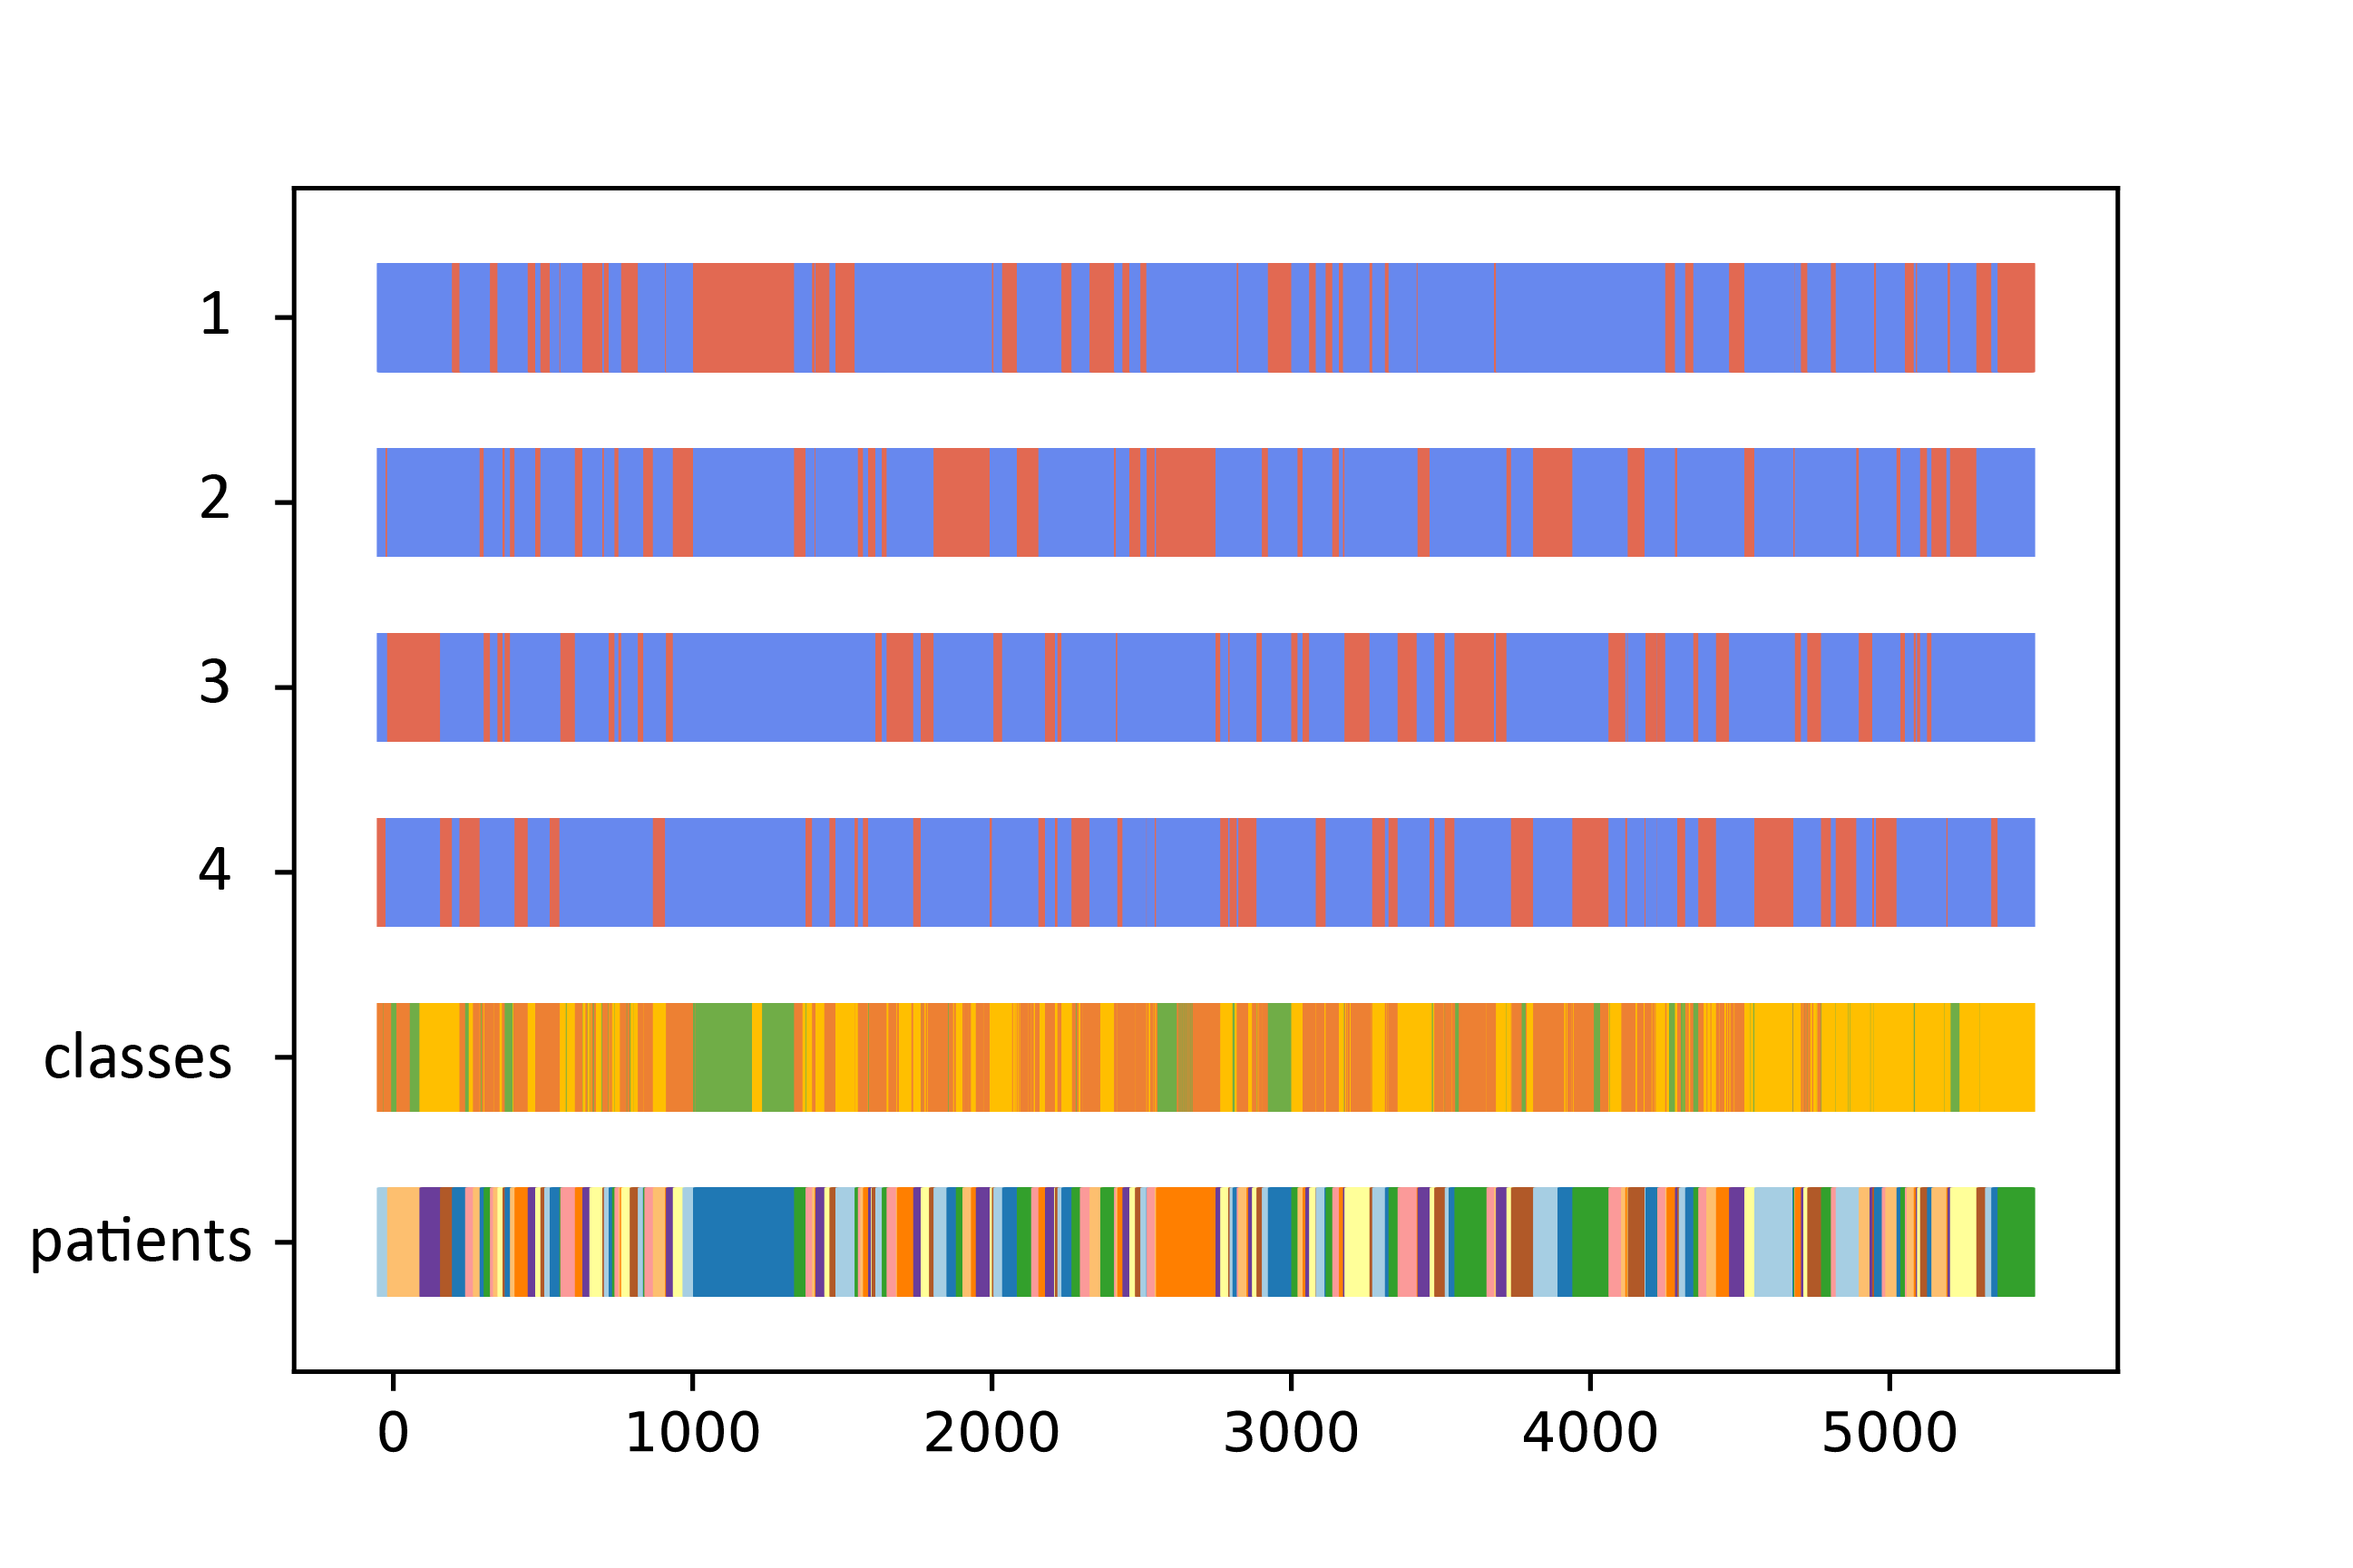
\includegraphics[width=0.8\linewidth]{contents/chapter_5/resources/visualisation_folds.png}
    \caption{Visualisation des divers lots d'évaluation utilisés pour l'évaluation des processus de classification.}
    \label{fig:visualisation_folds}
\end{figure}\par

Afin de régler les hyperparamètres et d'évaluer les performances des divers modèles, ce travail opte pour une métrique de type \fscore{} également discutée dans le \Cref{sec:models_settings}. En effet, cette métrique est robuste face à des déséquilibres d'annotations, tels que ceux rencontrés sur le jeu de données exploité. De plus, elle représente conjointement sous une unique mesure les valeurs de \textit{précision} et de \textit{rappel}. Son expression est binaire, elle sera ainsi calculée pour chaque classe dont la valeur est pondérée par le ratio du nombre d'échantillons disponibles dans chaque classe respective.\par

Ces expériences sont menées en plusieurs étapes successives, et débutent par l'évaluation de l'ensemble des méthodes d'extraction de caractéristiques conjointement à la normalisation de l'information selon la méthode de \textit{Minimum/Maximum} et la méthode \textit{Standard}. Aucun des tests menés n'est réalisé sur les caractéristiques brutes (sans normalisation), les expériences menées au préalable ne permettant pas de faire converger les modèles de classification dans un temps raisonnable de calcul.\par
 
\begin{figure}[H]
    \centering
    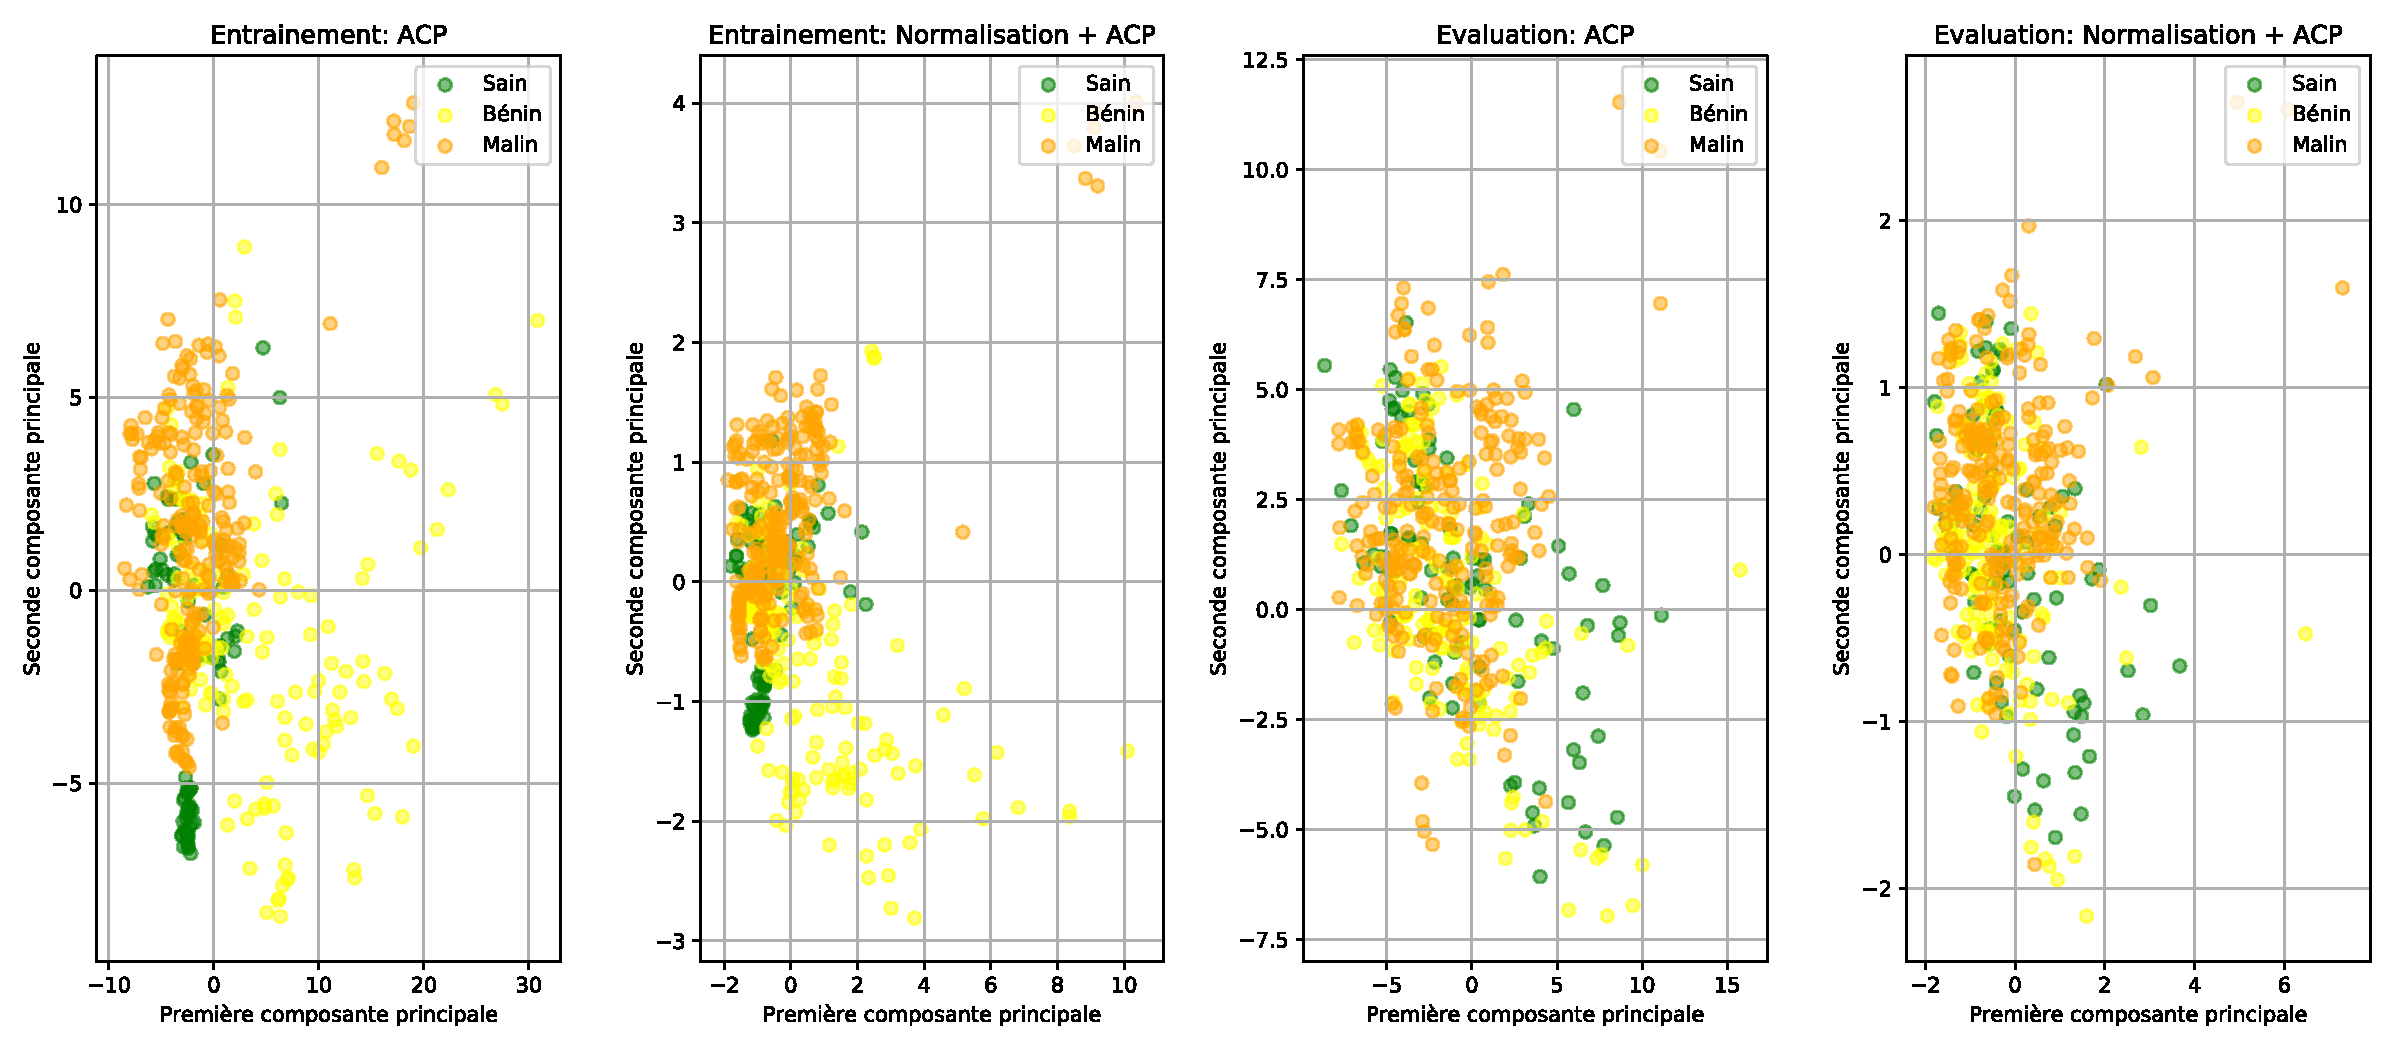
\includegraphics[width=\linewidth]{contents/chapter_5/resources/visualisation_scaling_PCA.pdf}
    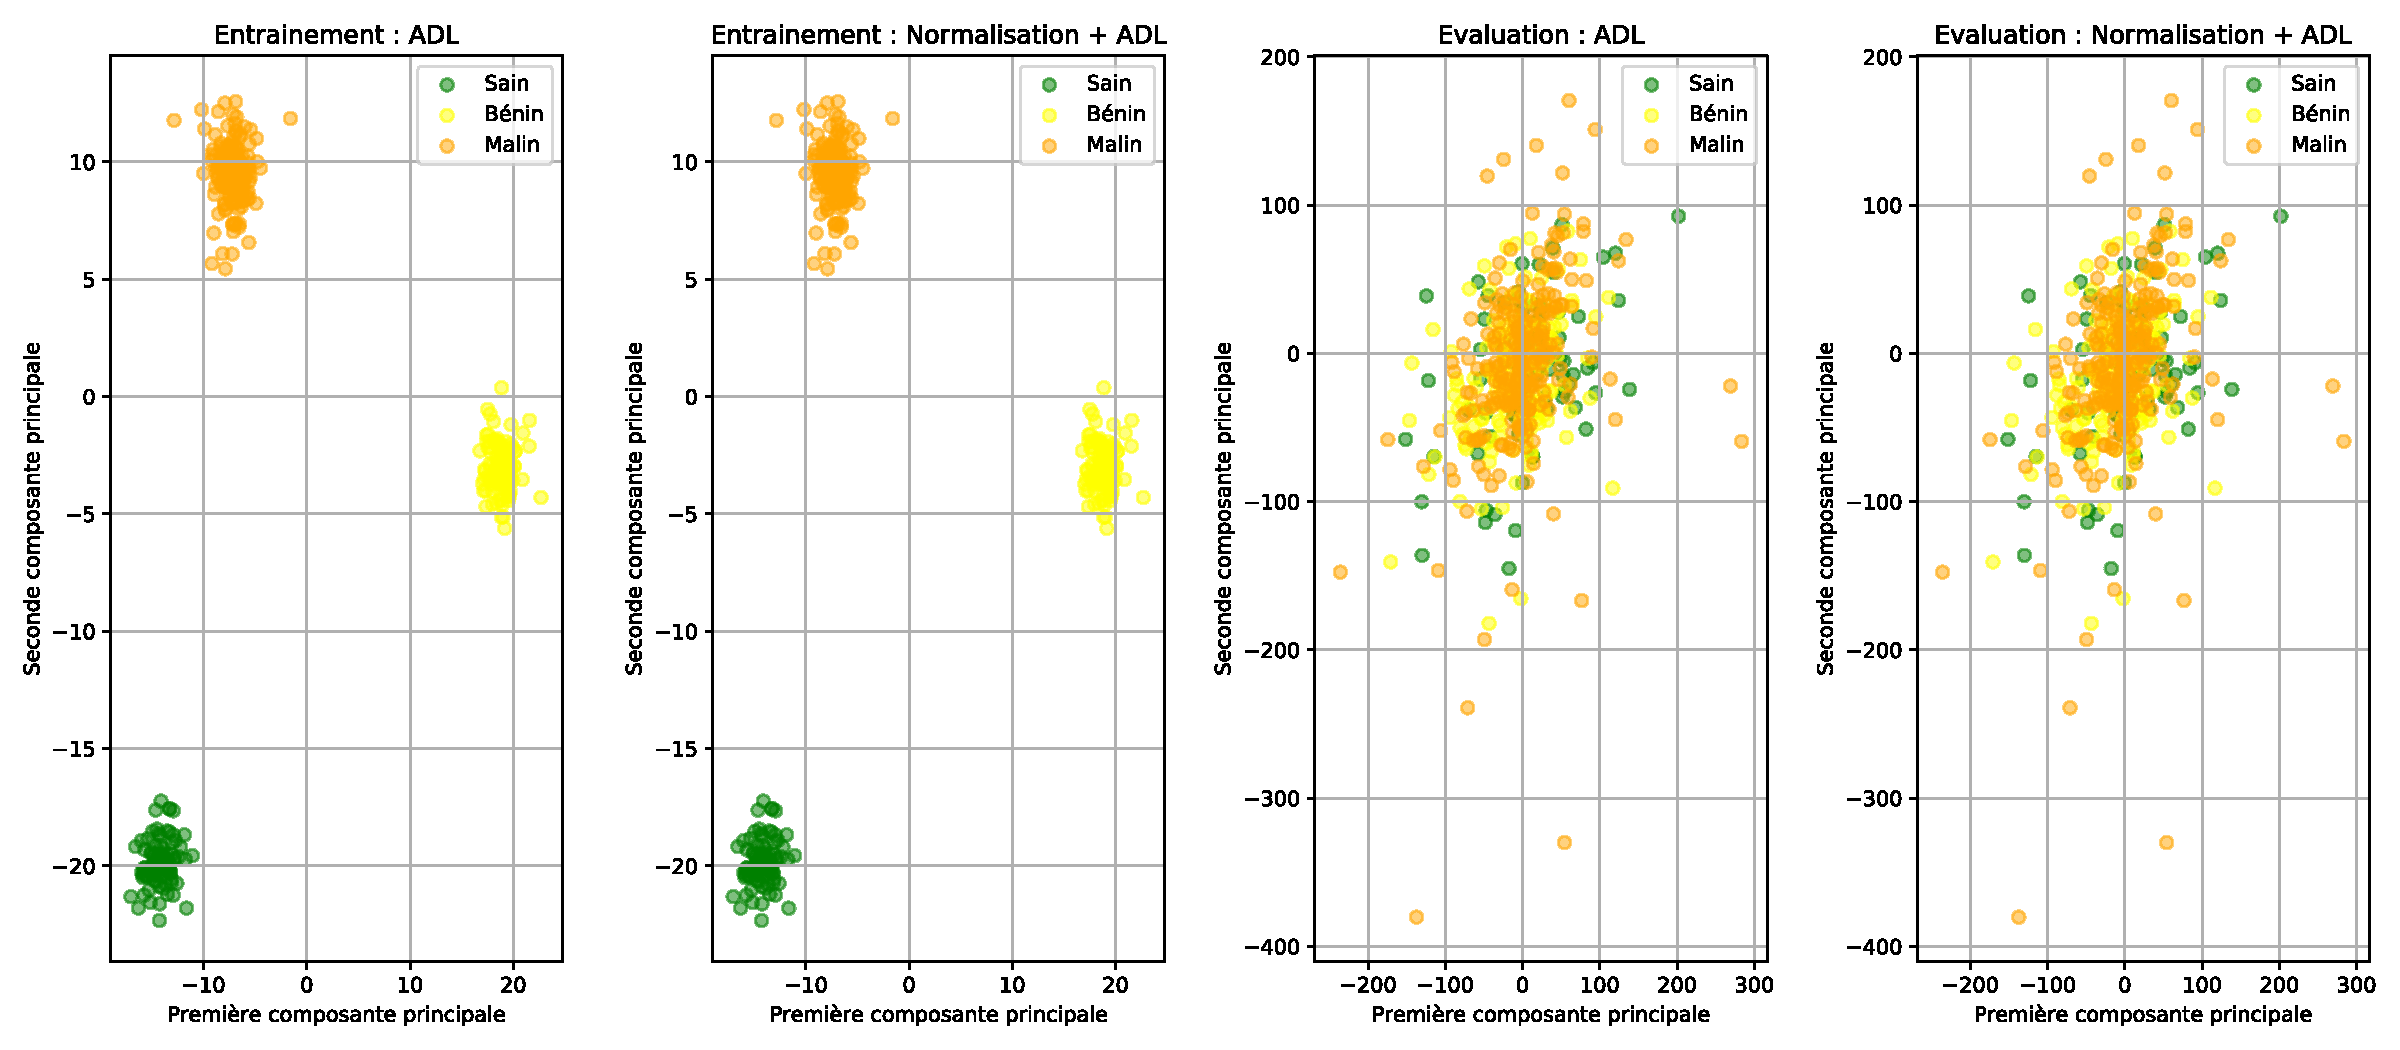
\includegraphics[width=\linewidth]{contents/chapter_5/resources/visualisation_scaling_LDA.pdf}
    \caption{Visualisation de l'influence de la réduction des dimensions appliquée au deux premières composantes principales, sur un échantillon constitué arbitrairement de 500 images issue des données de \gls{rcm} mise à disposition de ces travaux. En haut, technique de réduction basée sur le \gls{pca} ; En bas, technique de réduction basée sur le \gls{lda}. A gauche, un processus procédant à la réduction puis à la normalisation ; A droite, un processus procédant à la normalisation puis à la réduction.}
    \label{fig:visualisation_scaling_reduction}
\end{figure}\par

Puis, l'impact de la réduction de dimension est mesuré sur les techniques de transfert de connaissance avant de procéder à leur classification. Contrairement aux recommandations de la librairie~\textsuperscript{\ref{footnote:exemple_pca_scaling}}, ce travail adopte un schéma de type réduction de l'information suivi d'une normalisation de caractéristiques avant l'étape de classification. En effet, les caractéristiques issues de réseaux convolutionnels possèdent une distribution de valeurs consistantes, et n'affectent pas de manière significative les techniques de réduction de dimensions. En revanche, la réduction d'information par techniques de projection peut affecter la consistance de cette distribution des valeurs. Ce phénomène a notamment été observé sur un lot de 500 données choisies arbitrairement, et présentées sur la \Cref{fig:visualisation_scaling_reduction}.\par

Pour finir, ces expériences mesurent l'impact du déséquilibre des données sur les résultats de classification et évaluent la pertinence des méthodes qui visent à corriger ce déséquilibre dans ce contexte. Pour cela, les méthodes les plus pertinentes sont soumises à une classification sans correction du déséquilibre d'annotations mais également avec les divers mécanismes mentionnés dans la \Cref{subsec:balancement}, et leurs résultats sont comparés.\par

La sélection des modèles les plus pertinent se base sur les résultats à trois classes dans la mesure où ces scores sont représentatifs de la capacité à caractériser la problématique dans son ensemble. Néanmoins dans la dernière partie de cette analyse, seuls les résultats de la détection des images malignes sont détaillés dans la mesure où ceux-ci correspondent à l'objectif visé par ce travail.\par

\addtocounter{footnote}{1}
\footnotetext[\thefootnote]{Source~: Scikit-learn - \href{https://scikit-learn.org/stable/auto_examples/preprocessing/plot_scaling_importance.html}{«Importance of Feature Scaling»}. \label{footnote:exemple_pca_scaling}}
\clearpage

\section{Résultats}
Ce premier volet est mené sur les méthodes d'extraction de caractéristiques associées aux techniques de normalisation. Dans un premier temps, en terme de méthode d'extraction spatiale, un \fscore{} de 0,64 associé à un écart-type de 0,07 est obtenu par la méthode proposé par \textbf{Haralick} et al. et \textbf{sans moyenne des axes}. Ce score correspond à l'utilisation conjointe d'une normalisation de type \textbf{Minimum / Maximum} et d'un modèle \textbf{\gls{svm} avec un noyau à base radiale}. Dans un second temps, en terme de méthode d'extraction fréquentielle, un \fscore{} de 0,67 associé à un écart-type de 0,06 est obtenu par l'utilisation de l'extraction en \textbf{ondelettes de Daubechies}. Ce score correspond à l'utilisation conjointe d'une normalisation de type \textbf{Minimum / Maximum} et d'un modèle \textbf{\gls{svm} avec un noyau linéaire ou avec un noyau à base radiale}. De plus, ce score correspond également à l'utilisation conjointe d'une normalisation de type \textbf{Standard} et d'un modèle \textbf{\gls{svm} avec un noyau linéaire}. Enfin, en terme de méthode par transfert de connaissances, un \fscore{} de 0,77 associé à un écart-type de 0,04 est obtenu sur l'architecture \textbf{ResNet-50} combinée à une couche de \textbf{Global Pooling - Moyen}. Ce score correspond à l'utilisation conjointe d'une normalisation de type \textbf{Minimum / Maximum} et d'un modèle \textbf{\gls{svm} avec un noyau linéaire}. L'ensemble des résultats liés à ces expérimentations est visible sur la \Cref{fig:results_image_classification}.\par

\begin{figure}[H]
    \centering
    
    \begin{subfigure}{\textwidth}
      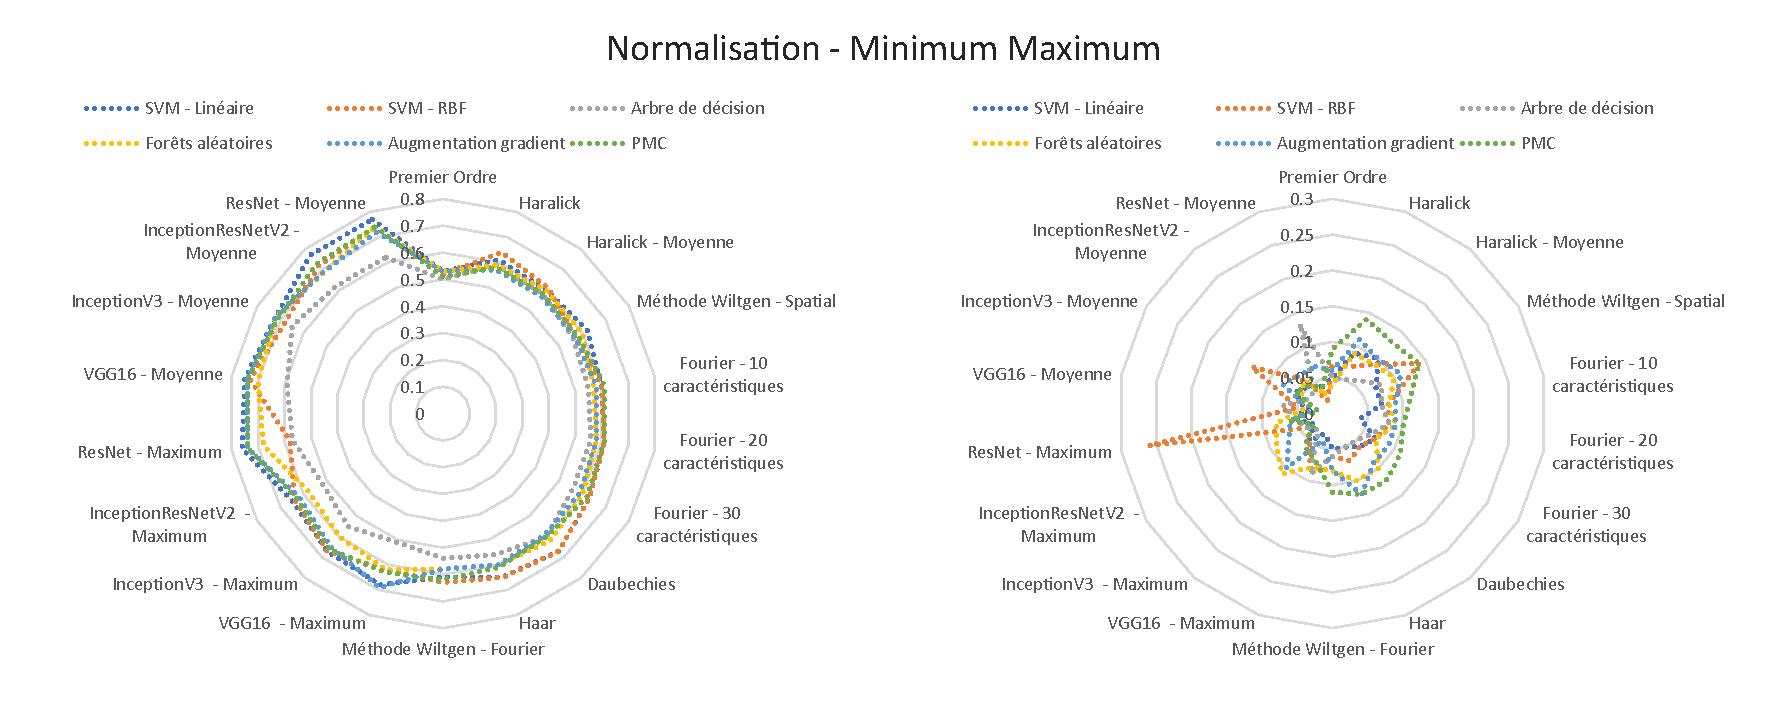
\includegraphics[width=\textwidth]{contents/chapter_5/resources/results_image_classification_mms.pdf}
    \end{subfigure}
    
    \begin{subfigure}{\textwidth}
      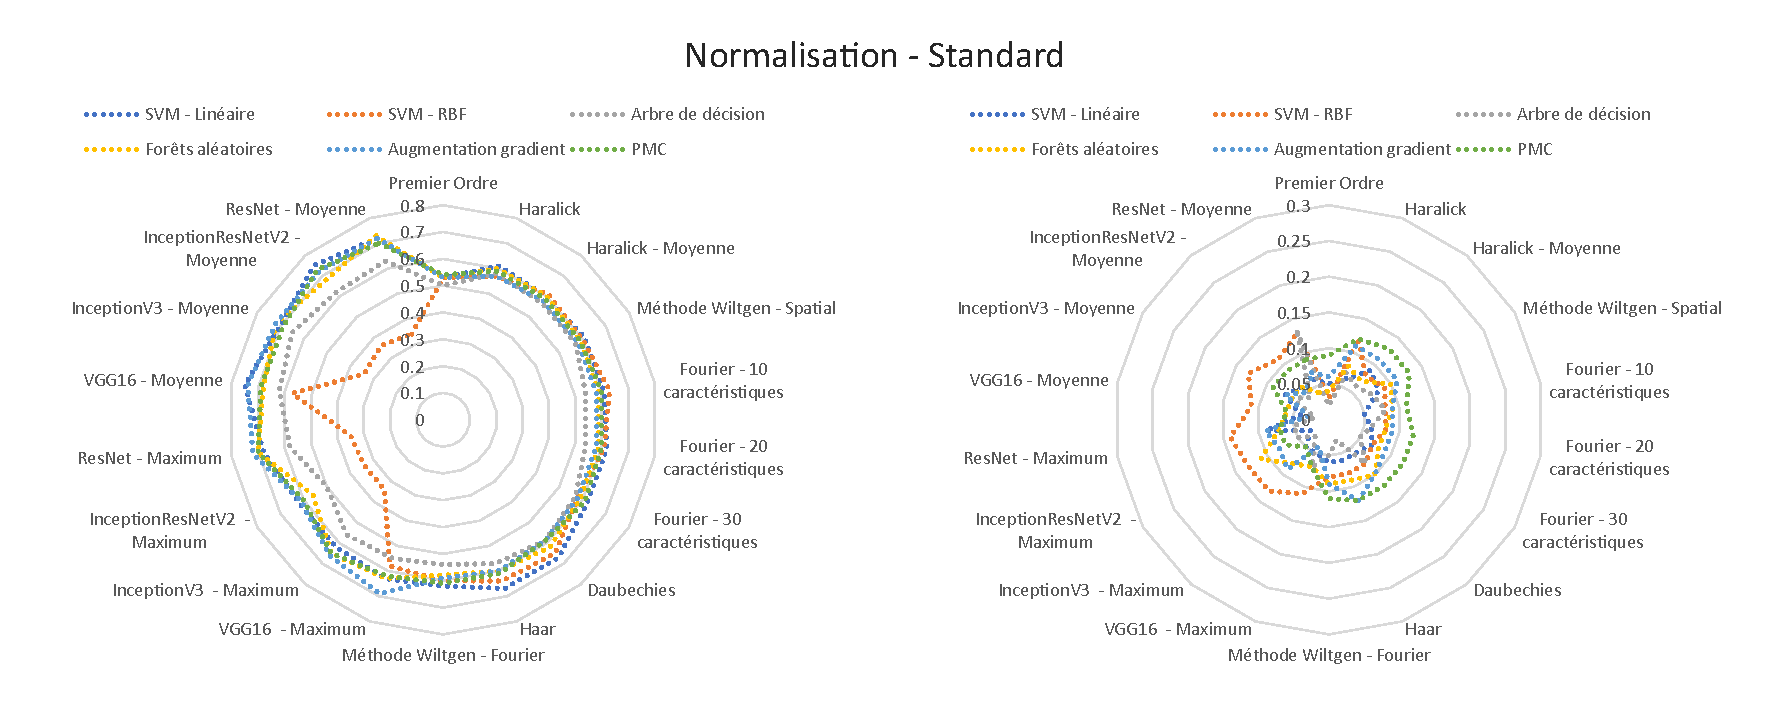
\includegraphics[width=\textwidth]{contents/chapter_5/resources/results_image_classification_ss.pdf}
    \end{subfigure}
    
    \caption{Résultats issus de la classification par les diverses techniques d'extraction et par les modèles de classification mentionnés en couleur. En haut, les résultats provenant de la normalisation de type \textit{Minimum / Maximum} ; En bas, les résultats provenant de la normalisation de type \textit{Standard}. A gauche, la représentation basée sur les valeurs moyennes ; A droite, la représentation tenant compte de l'écart-type.}
    \label{fig:results_image_classification}
\end{figure}\par

Ce second volet mesure l'impact de la réduction d'informations sur les méthodes d'extraction par transfert de connaissances. En effet, la grande quantité d'informations issues de ces techniques peut provoquer une dégradation des performances de classification, ce que tente de vérifier ce nouveau paragraphe. Seules les architectures couplées à une couche de \textit{Global Pooling - Moyen} sont évaluées, leurs performances ayant été significativement supérieures aux architectures couplées avec un \textit{Global Pooling - Maximum}. D'une part, un \fscore{} de 0,76 associé à un écart-type de 0,03 est obtenu sur l'architecture \textbf{ResNet-50} combinée à une couche de \textbf{Global Pooling - Moyen}. Ce score provient de l'utilisation conjointe de \textbf{l'\gls{pca} avec une variance cumulée de 99\%}, d'une normalisation de type \textbf{Minimum / Maximum} et d'un modèle \textbf{\gls{svm} avec un noyau linéaire}. D'autre part, un \fscore{} de 0,73 associé à un écart-type de 0,05 est obtenu sur l'architecture \textbf{VGG-16} combinée à une couche de \textbf{Global Pooling - Moyen}. Ce score provient de l'utilisation conjointe de \textbf{l'\gls{lda} avec une variance cumulée de 95\%}, d'une normalisation de type \textbf{Standard} et d'un modèle \textbf{\gls{svm} avec un noyau linéaire}. Les résultats de ce volet de l'expérience sur les méthodes de réduction de l'information sont reportés sur la \Cref{fig:results_image_classification_reduction}.\par

\begin{figure}[H]
    \centering
    
    \begin{subfigure}{\textwidth}
      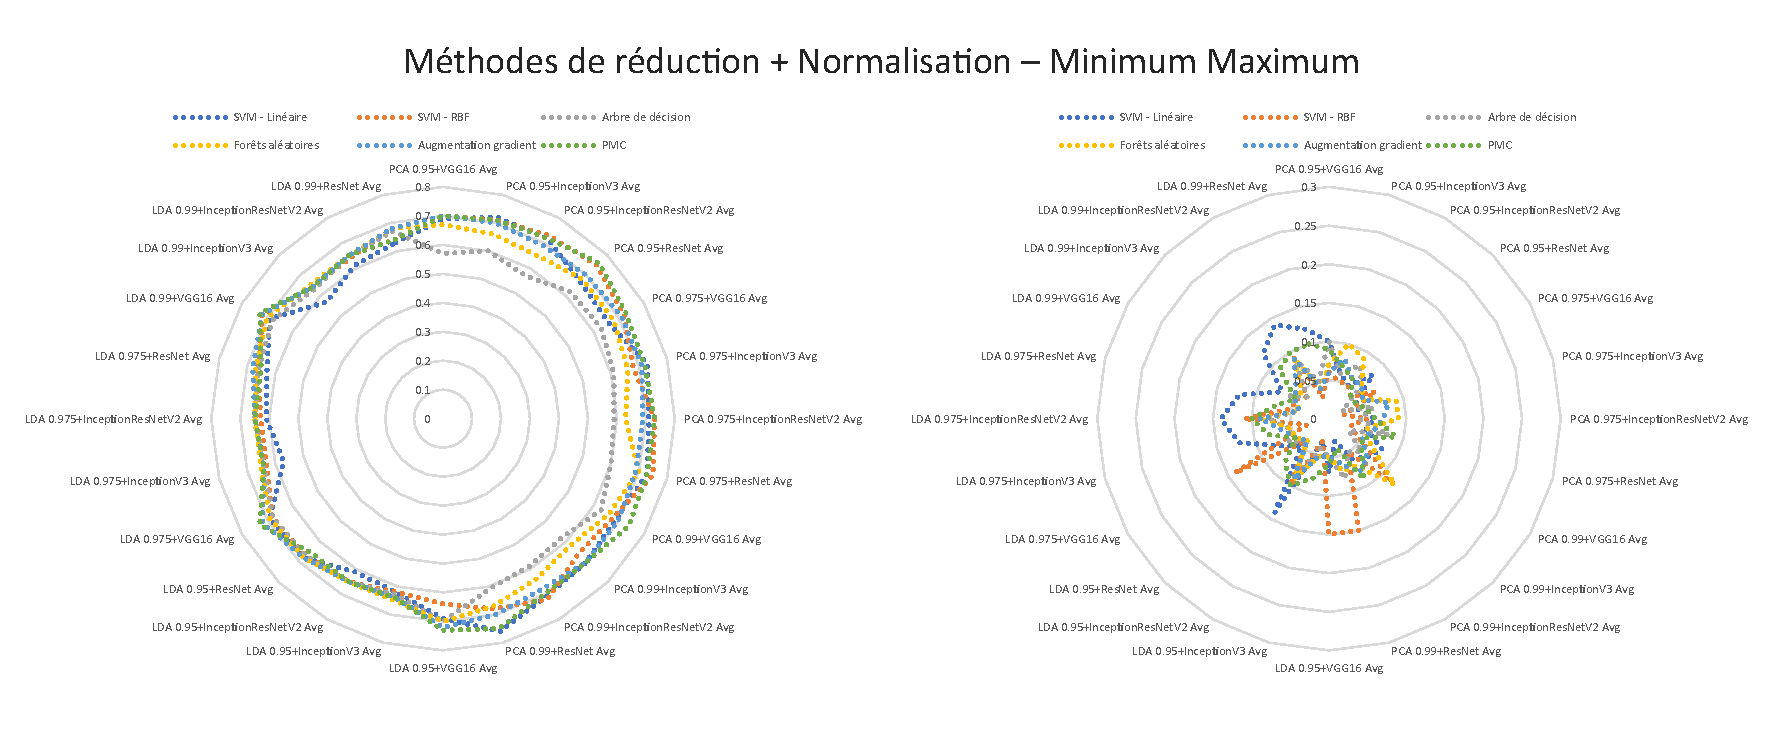
\includegraphics[width=\textwidth]{contents/chapter_5/resources/results_image_classification_reduction_mms.pdf}
    \end{subfigure}
    
    \begin{subfigure}{\textwidth}
      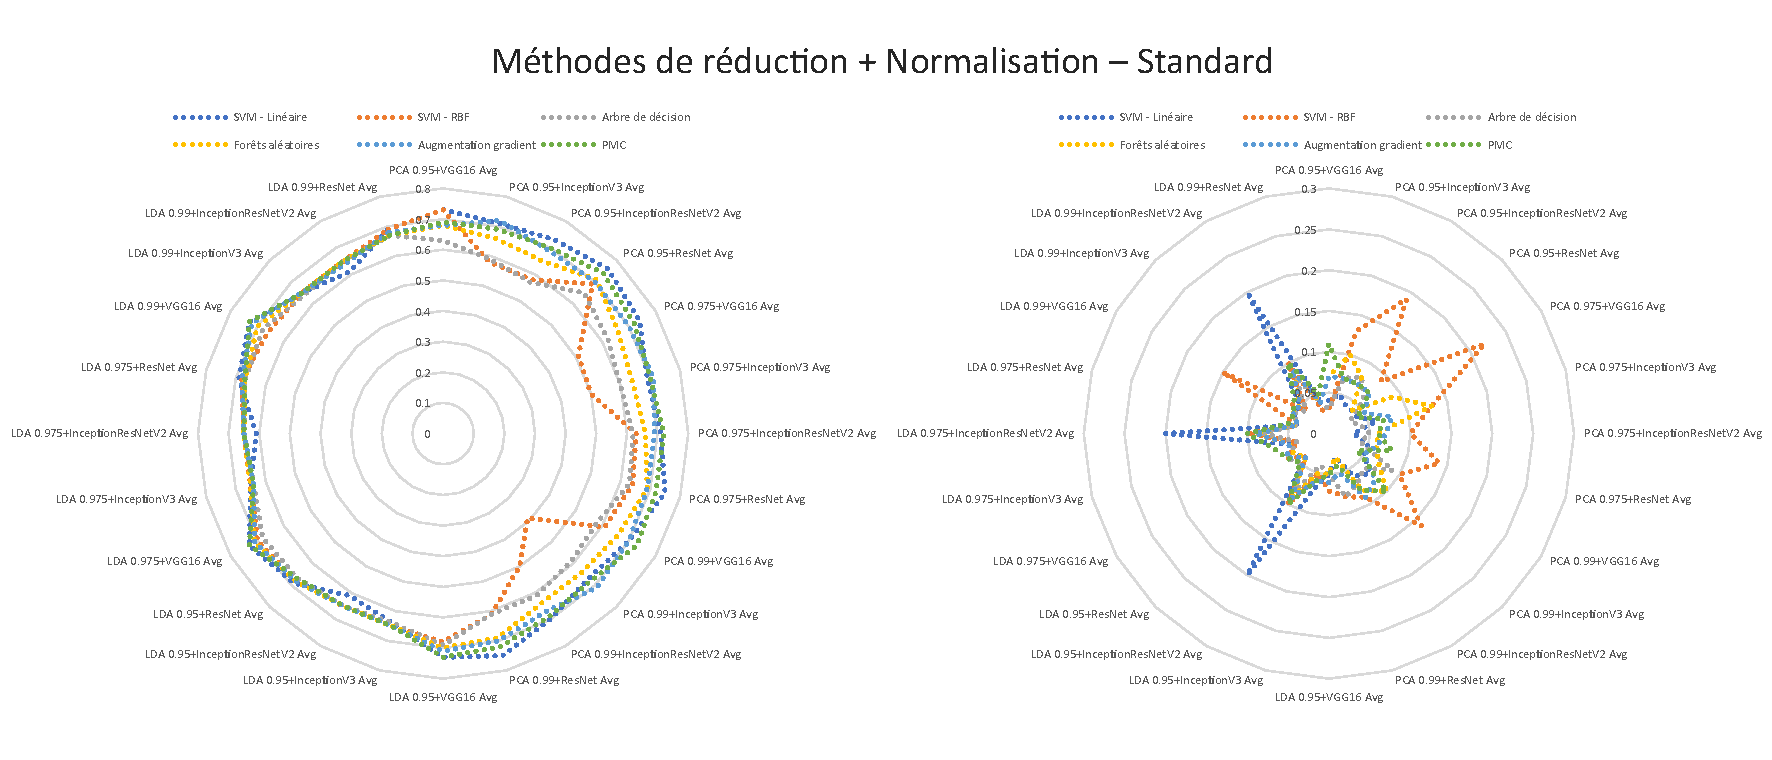
\includegraphics[width=\textwidth]{contents/chapter_5/resources/results_image_classification_reduction_ss.pdf}
    \end{subfigure}
    
    \caption{Résultats issus de la classification par l'utilisation de techniques de réduction combinés aux techniques d'extraction par transfert et, par les modèles de classification mentionnés en couleur. Les tracés de couleurs représentent les divers modèles évalués au cours de l'expérience. En haut, les résultats provenant de la normalisation par Minimum/Maximum ; En bas, les résultats provenant de la normalisation par score Standard. A gauche, la représentation basée sur les valeurs moyennes ; A droite, la représentation tenant compte de l'écart-type.}
    \label{fig:results_image_classification_reduction}
\end{figure}\par

Le dernière volet de ces expérimentations se destine à étudier l'impact du déséquilibre des données sur la qualité des résultats de classification. Son influence est mesuré sur les méthodes les plus performantes relatives aux précédents paragraphes de cette section, couplé aux méthodes de corrections de ces déséquilibres. Ainsi, un \fscore{} de 0,77 associé à un écart-type de 0,04 est obtenu par la méthode de transfert de connaissances basée sur l'architecture \textbf{ResNet-50} couplé à une couche de \textbf{Global Pooling - Moyen}. Ce score résulte de l'utilisation conjointe d'une normalisation \textbf{Minimum/Maximum} suivi d'un modèle \textbf{\gls{svm} à noyau linéaire} dont l'utilisation est combinée à l'utilisation \textbf{d'une pondération} dans le but de compenser le déséquilibre de données. Les résultats lié à l'étude du déséquilibre des données à trois classes sont visibles sur la \Cref{tab:results_balancement_multi}.\par

\begin{table}[H]
    \begin{tabular}{lllllll}
        \toprule
                    & Aucune        & Pond.                 & Sur-éch.      & Sous-éch.     & SMOTE+ENN     & SMOTE+Tomek   \\ \hline
        Spatial     & 0,55$\pm$0,15 & 0,61$\pm$0,09         & 0,54$\pm$0,15 & 0,58$\pm$0,11 & 0,60$\pm$0,09 & 0,56$\pm$0,16 \\
        Fréquentiel & 0,59$\pm$0,13 & 0,67$\pm$0,06         & 0,55$\pm$0,21 & 0,58$\pm$0,17 & 0,61$\pm$0,12 & 0,64$\pm$0,10 \\ \rowcolor[HTML]{E7E6E6}
        Transfert   & 0,71$\pm$0,08 & \textbf{0,77$\pm$0,04}& 0,74$\pm$0,07 & 0,72$\pm$0,05 & 0,74$\pm$0,05 & 0,74$\pm$0,05 \\
        Réduction   & 0,71$\pm$0,09 & 0,76$\pm$0,03         & 0,74$\pm$0,06 & 0,73$\pm$0,04 & 0,73$\pm$0,04 & 0,73$\pm$0,06 \\ \bottomrule
    \end{tabular}
    \caption{Résultats à trois classes issus de l'expérience mêlant les méthodes les plus performantes associée aux méthodes de balancement de données évoquées.}
    \label{tab:results_balancement_multi}
\end{table}\par

Ces même résultats sont également observés du point de vue des performances de la classe maligne. Par ce nouveau point de vue, un \fscore{} de 0,82 associé à un écart-type de 0,02 est obtenu par la méthode de transfert de connaissances basée sur l'architecture \textbf{ResNet-50} couplé à une couche de \textbf{Global Pooling - Moyen}. Comme précédemment, ce score résulte de l'utilisation conjointe d'une normalisation \textbf{Minimum/Maximum} suivi d'un modèle \textbf{\gls{svm} à noyau linéaire} dont l'utilisation est combinée à l'utilisation \textbf{d'une pondération} dans le but de compenser le déséquilibre de données. Les résultats lié à l'étude du déséquilibre des données, et adoptant le point de vue de la classe maligne, sont disponibles sur la \Cref{tab:results_balancement_malignant}.\par

\begin{table}[H]
    \begin{tabular}{lllllll}
        \toprule
                    & Aucune        & Pond.                 & Sur-éch.      & Sous-éch.     & SMOTE+ENN     & SMOTE+Tomek   \\ \hline
        Spatial     & 0,65$\pm$0,11 & 0,63$\pm$0,07         & 0,64$\pm$0,10 & 0,64$\pm$0,08 & 0,63$\pm$0,09 & 0,59$\pm$0,27 \\
        Fréquentiel & 0,70$\pm$0,09 & 0,68$\pm$0,03         & 0,66$\pm$0,09 & 0,66$\pm$0,09 & 0,61$\pm$0,22 & 0,66$\pm$0,09 \\ \rowcolor[HTML]{E7E6E6} 
        Transfert   & 0,81$\pm$0,04 & \textbf{0,82$\pm$0,02}& 0,81$\pm$0,03 & 0,79$\pm$0,01 & 0,80$\pm$0,02 & 0,82$\pm$0,03 \\
        Réduction   & 0,81$\pm$0,03 & 0,81$\pm$0,01         & 0,81$\pm$0,03 & 0,79$\pm$0,03 & 0,80$\pm$0,01 & 0,81$\pm$0,03 \\ \bottomrule 
    \end{tabular}
    \caption{Résultats de la détection de tissus malins issus de l'expérience mêlant les méthodes les plus performantes associées aux méthodes de balancement de données évoquées.}
    \label{tab:results_balancement_malignant}
\end{table}\par

Enfin, les courbes \gls{roc} permettent d'appréhender les performances de prédiction de ce système. Ainsi, les performances propres à l'ensemble de la base d'images annotées sont homogènes par cette technique avec des scores \gls{auc} dont les valeurs sont comprises entre 0,87 et 0,90, Néanmoins, une analyse \gls{roc} des lésions de types \gls{lm} et \gls{lmm} comme seules représentantes des classes malignes mettent en avant des performances moins homogènes entre les diverses classes. Ces scores \gls{auc} dont les valeurs varient entre 0,79 et 0,92 représentent une limite de ces méthodes a différencier les tissus bénins et les tissus malins. Ces diverses courbes sont visibles sur la \Cref{fig:results_image_classification_roc}.\par

\begin{figure}[H]
    \centering
    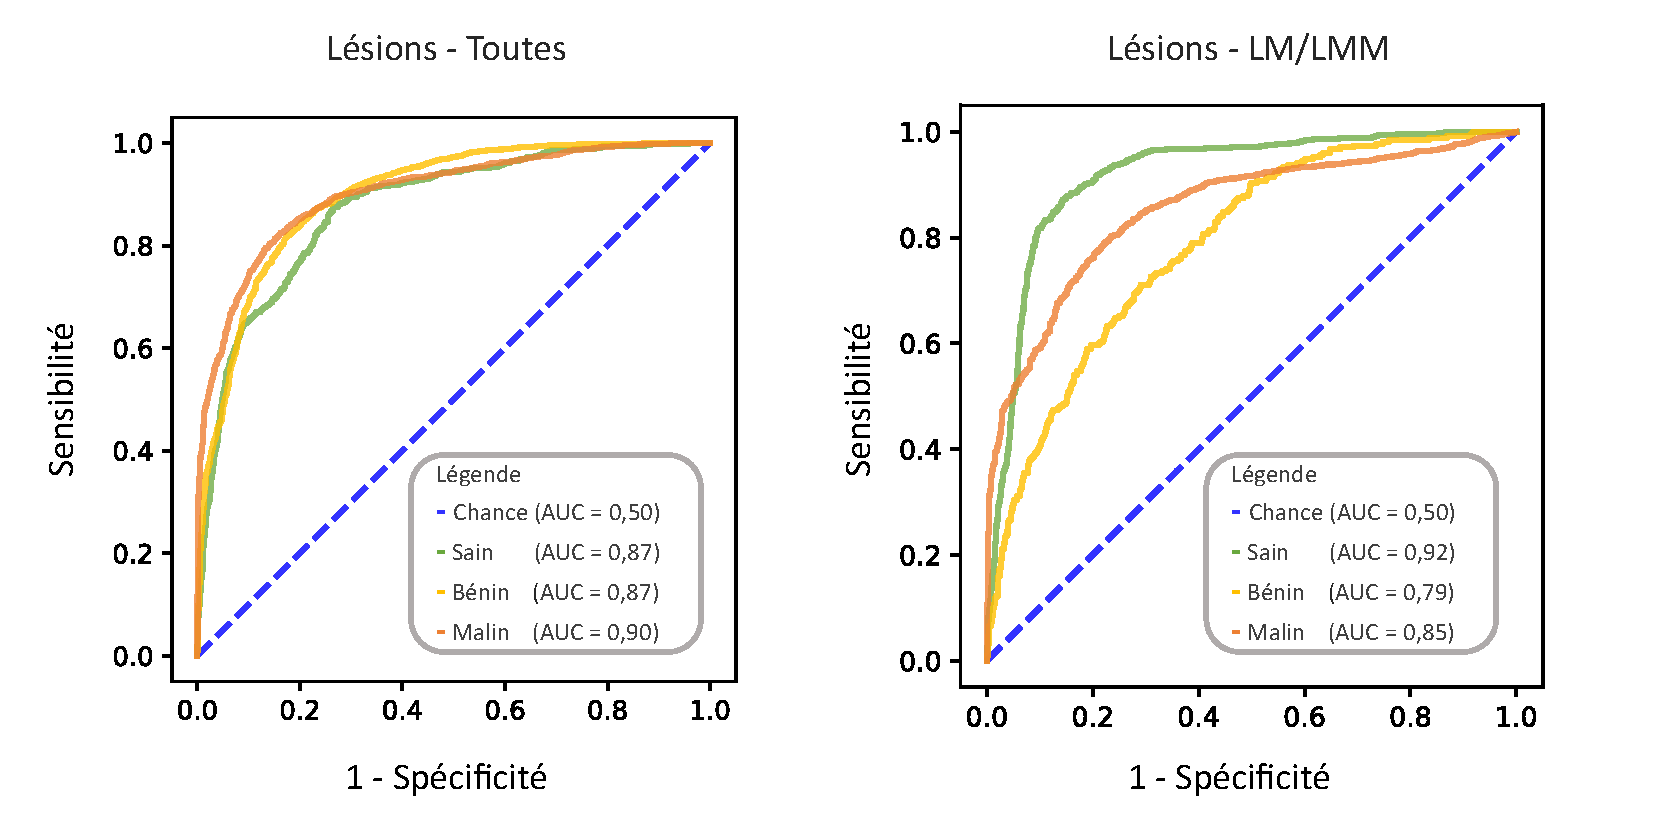
\includegraphics[width=\textwidth]{contents/chapter_5/resources/results_image_classification_roc.pdf}
    \caption{Résultats sous forme de courbes \gls{roc}. A gauche, résultats sur l'ensemble des lésions d'étude ; A droite, résultats excluant les lésions malignes différentes des types \gls{lm}/\gls{lmm}.}
    \label{fig:results_image_classification_roc}
\end{figure}\par

\section{Discussion}
Suite aux précédents résultats, plusieurs constats peuvent être formulés pour donner suite à la mise en pratique des méthodes d'extraction de caractéristiques. Le premier constat concerne les méthodes d'extraction spatiales, et plus particulièrement l'utilité de la méthode proposée par Haralick et al. sur les données de \gls{rcm} utilisées dans ce travail. En revanche, l'ajout de mesures de premier ordre ne semble pas ou peu impacter les performances. Le second constat concerne les méthodes d'extraction fréquentielles, et en particulier la supériorité sur ces données de l'extraction de caractéristiques par la transformée en ondelettes comparé à l'extraction de caractéristiques par la transformée de Fourier. Ce travail à également confirmé la faible influence de l'ondelette mère sur ces même données, bien que l'ondelette mère de Daubechies soit plus performante dans ce travail. Enfin, le dernier constat concerne la proposition de méthodes sur la base de transfert de connaissance à partir d'architectures de \gls{cnn} pré-entraînées, dont les résultats sont significativement supérieurs aux autres méthodes. Sur l'ensemble des architectures évaluées, la combinaison mêlant l'architecture ResNet-50 pré-entraîné sur ImageNet à une couche de \textit{Global Pooling - Moyen} produit les résultats les plus pertinent et sont plus amplement développée dans la suite de ce travail.\par

En termes de modèles de classification, l'un de ces constats concerne le modèle \gls{svm} avec noyau linéaire dont les performances et la stabilité sont les plus pertinentes dans la plupart des expériences menées lors de ce chapitre. Par opposition, le modèle \gls{svm} avec noyau à base radiale a été essentiellement pertinent à l'aide d'une normalisation par Minimum / Maximum, sa performance et stabilité chutant de manière drastique lorsque les caractéristiques sont nombreuses. Du côté des méthodes basées sur les arbres de décision, ces techniques sont globalement peu influencées par les méthodes de normalisation. Comme attendu, les \gls{cart} sont performants dans la plupart des situations, exceptées celles par transfert de connaissances dans lesquelles le nombre de caractéristiques est trop important. A cette fin, les techniques de \gls{rf} et \gls{gb} ont été particulièrement adaptées, les \gls{gb} étant légèrement moins stables que les \gls{rf}. Pour finir cette analyse des modèles, l'utilisation de \gls{mlp} dans le but d'observer l'effet de la non-linéarité semble ne pas avoir aidé à améliorer la classification.\par

Afin de compenser le nombre élevé de caractéristiques extraites par les \gls{cnn}, des techniques de réduction mises en place afin de pallier ce problème sont évaluées. Dans ce travail, leur utilisation réduit les performances de prédiction mais également la stabilité en augmentant sensiblement l'écart-type. Bien que moins performants, des résultats intéressants sont obtenues dans une configuration utilisant ResNet-50 et l'\gls{pca} avec une variance expliquée de 99\% permettant de retirer près des trois quarts des caractéristiques. La relation entre variance expliquée et caractéristiques par cette méthode est visible sur la \Cref{fig:results_image_classification_pca_variance}.\par

\begin{figure}[H]
    \centering
    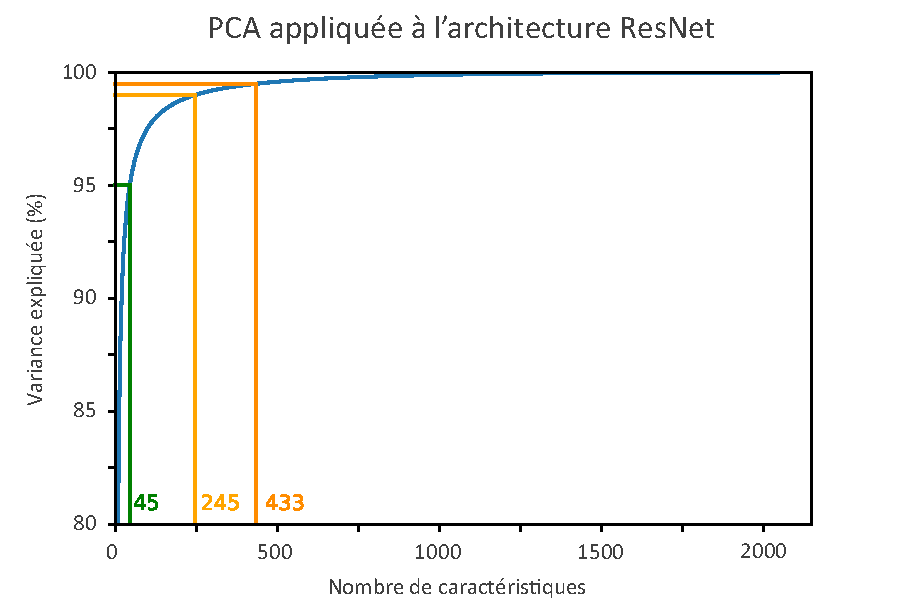
\includegraphics[width=0.8\textwidth]{contents/chapter_5/resources/results_image_classification_pca_variance.pdf}
    \caption{Analyse de la variance expliquée cumulée par l'application de l'\gls{pca}. Le nombre de caractéristiques est représenté pour des variances expliquées de 95\% en vert, 99\% en jaune et 99,5\% en orange.}
    \label{fig:results_image_classification_pca_variance}
\end{figure}\par

La dernière méthode mise en œuvre pour optimiser les performances de classification des images concerne le balancement des annotations. Dans le contexte de ce manuscrit, la méthode par pondération est préférée aux autres méthodes de sa catégorie car elle propose une correction du non-balancement à moindre frais, tout en garantissant de meilleure performances sur l'ensemble des expériences menées.\par

En conclusion, ce premier chapitre expérimental a permis de mettre au point un processus permettant de traiter les données \gls{rcm}. Les expérimentations menées permettent d'accomplir une classification avec un \fscore{} de 0,77 associé à un écart-type de 0,04 pour 3 classes et de 0,82 associé à un écart-type de 0,02 pour la classification d'éléments malins. De plus ce processus a permis l'obtention d'une \gls{auc} de 0,90 sur l'ensemble des données et de 0,85 sur les données excluant les lésions différentes des types \gls{lm} et \gls{lmm}. Néanmoins, des améliorations sur la qualité de ce processus de diagnostic sont à prévoir, ainsi que sur la possible prise en compte de l'intersection d'évènements tels que la présence de tissus caractéristiques auprès de follicules pileux.\par